\renewcommand{\thechapter}{\Roman{chapter}}
\chapter{Result and Discussion}
\renewcommand{\thechapter}{\arabic{chapter}}
\label{ch:Result and Discussion}
\thispagestyle{empty}

The results of the system development outlined in the previous chapter were presented and discussed in this chapter. After evaluating the specification of each system and undergo different design revision and integration, the study successfully identified and finalized the necessary components, tools and materials for each system.

\section{3D Point Cloud Scanner System}

% \subsection{3D-PCSS CAD Design Setup}

The CAD Design of 3D Point Cloud Scanner System setup, as shown in figure \ref{ch4:fig:cad_storage_bin}, consists of a 2D LiDAR Device fixed to a platform connected to a servo motor. This servo motor allows the platform to rotate, giving the LiDAR device an extra axis of movement. The 2D LiDAR device and servo motor used in this study are the YDLiDAR X4 Model and AX12A Dynamixel servo motor respectively. The detailed specification of each of the components is presented in appendix \ref{appen:a}.

Inside the compartment is where the single-board computer along with other circuit components located. The system is powered by a battery Inside the compartment, the specific components and its category is shown in figure \ref{ch4:fig:specific-components} and the system is powered by a battery. \\

\begin{figure}[H]
	\centering
	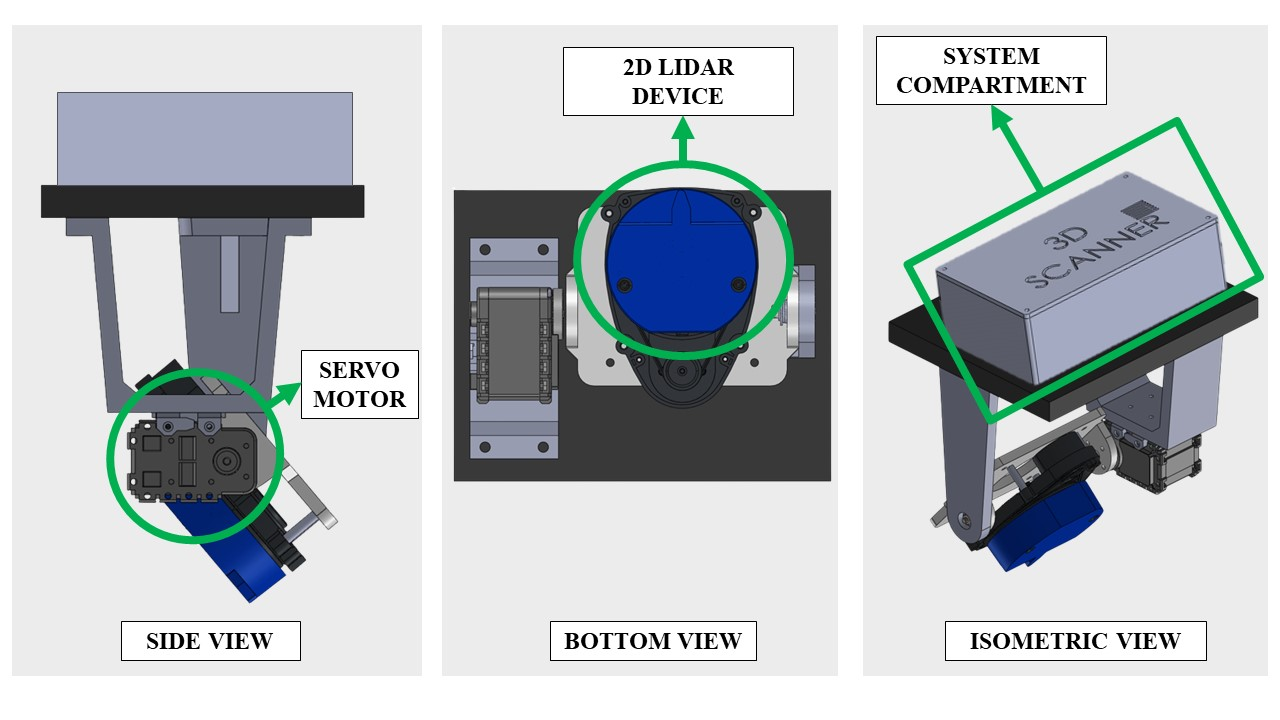
\includegraphics[width=1\textwidth]{Figures/3d-pcss-cad-design}
	\caption{Different View of the CAD Model Design of 3D Point Cloud Scanner System}
	\label{ch4:fig:cad_storage_bin}
\end{figure}

\begin{figure}[H]
	\centering
	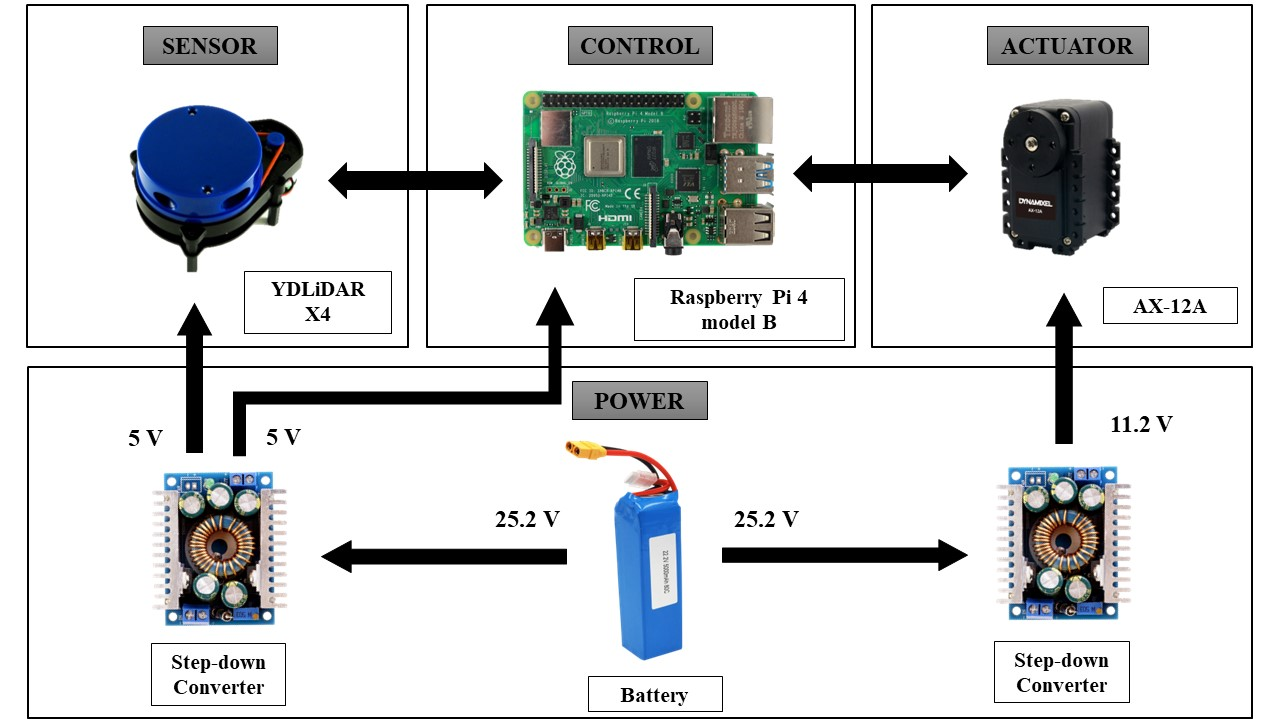
\includegraphics[width=1\textwidth]{Figures/specific-components}
	\caption{Specific Components of the System}
	\label{ch4:fig:specific-components}
\end{figure}

% \subsection{System Hardware}

\subsection{Actual Prototype of the 3D Point Cloud Scanner System}

The actual 3D Point Cloud Scanner System developed is shown in figure \ref{ch4:fig:actual-3d-pcss} was constructed in accordance with the 3D CAD model design. Before the integration of the system, individual component testing were conducted to test and verify if such components function properly. The base platform, to which the 2D LiDAR device and servo motor are attached, was fabricated using aluminum metal. The system compartment was 3D printed. Figure \ref{ch4:fig:circuit-diagram} shows the circuit diagram of the system. \\
\begin{figure}[H]
	\centering
	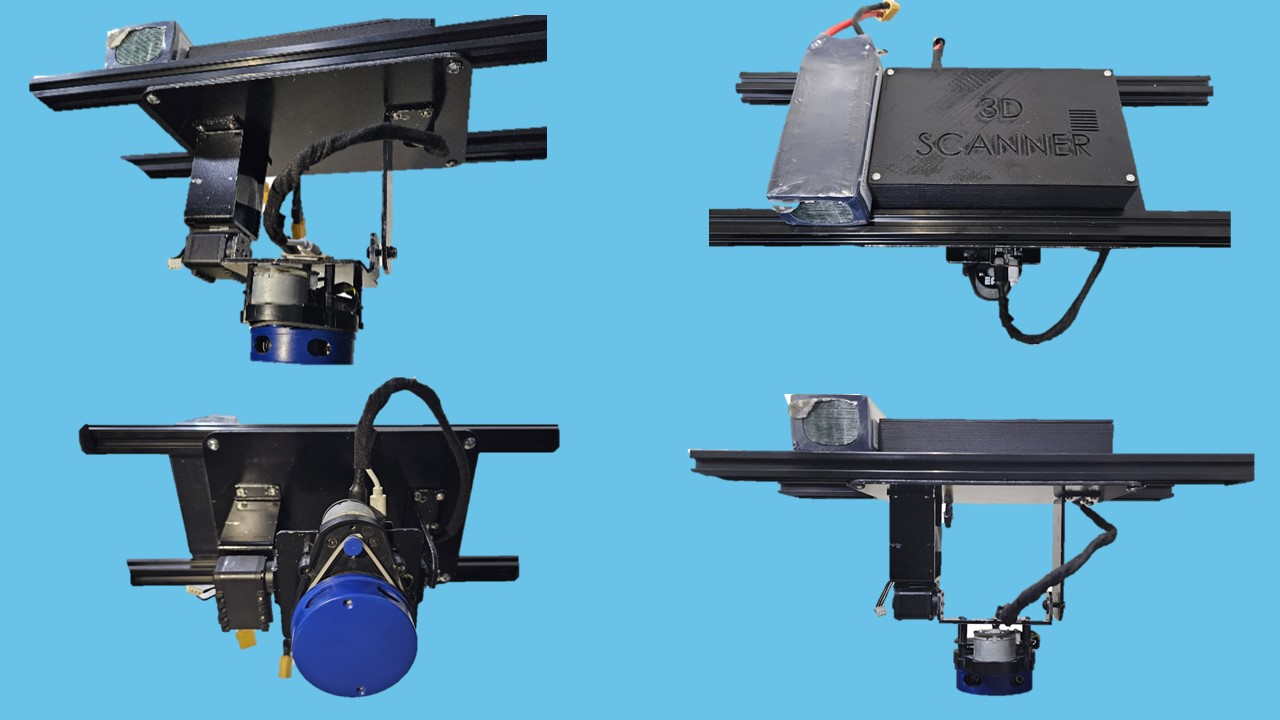
\includegraphics[width=1\textwidth]{Figures/actual-3d-pcss}
	\caption{Actual 3D Point Cloud Scanner System Developed}
	\label{ch4:fig:actual-3d-pcss}
\end{figure}

\begin{figure}[H]
	\centering
	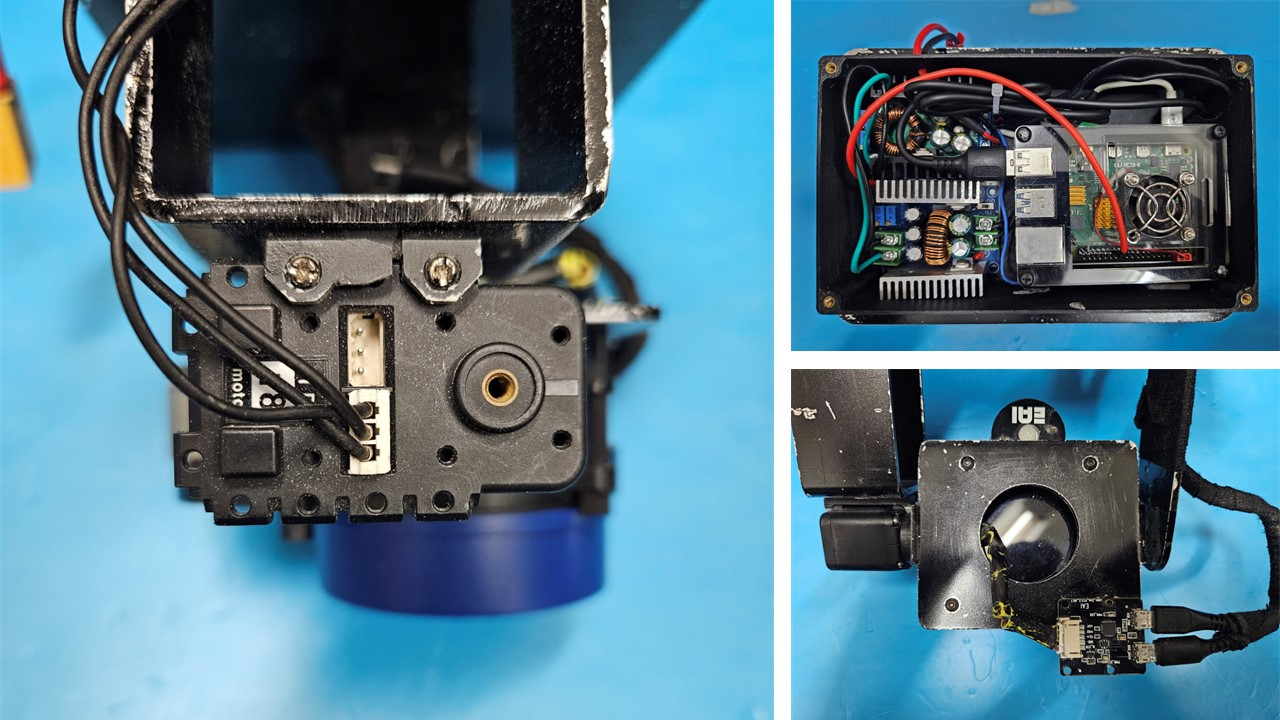
\includegraphics[width=0.9\textwidth]{Figures/actual-circuit-components}
	\caption{Actual Circuit Components of the System}
	\label{ch4:fig:circuit-diagram}
\end{figure}

\subsection{Software Development Result}

The processes of the system discussed in section \ref{ch3:subsec:software-development} were implemented on the single-board computer (Raspberry Pi 4 model B), which serves as the central component driving the functionality of the 3D Point Cloud Scanner System.

The figure \ref{ch3:fig:nodes-topics-relationships} demonstrated in chapter 3 illustrates the developed processes of the system, structured around a publish-subscribe model, facilitating efficient communication and data exchange between different nodes. The arrows in the diagram show how data flows between the different nodes and its relationship to a corresponding topics. The ROS bridge server Node facilitates communication by relaying commands between the web application and the ROS framework via the \texttt{/rosapi} service. Commands to start and stop scanning from the web interface are processed using the Remote Command Node within the system. The LiDAR Node captures ranges data and publishes it as distance values (meter), while the Dynamixel Node and LiDAR Node synchronize their operations through the \texttt{/dxl\_pos} topic. The Scan to 3D Point Cloud Mapping Node converts raw scan data into usable 3D point cloud data. The data type associated with the topics provdied such as \texttt{/raw\_point\_cloud} and \texttt{/processed\_pc} comprise a structured format, representing individual data points in three-dimensional space. Attributes within this data structure include spatial coordinates (e.g., X, Y, Z), intensity values, angles, and timestamps. The post-processing stage refines the point cloud data for volume measurement. Lastly, the expected value from the topic \texttt{/measured\_volume} corresponds to the volumetric value express in cubic meters ($m^3$) which is from the calculated volume of Convex hull.

Figure \ref{ch4:fig:volume-estimation-example} illustrates an example of the developed volume estimation process of teh system. The raw data from the LiDAR is converted into point cloud data. This point cloud data can then use the convex hull to create a mesh for volume estimation. The Quickhull algorithm used for this process is shown algorithm \ref{alg:quickhull3d}.

\begin{algorithm}[H]
	\caption{Quickhull Algorithm for 3D Point Cloud Volume Calculation}
	\label{alg:quickhull3d}
	\begin{algorithmic}[1]
		\REQUIRE Point cloud data $P$
		\ENSURE Convex hull $H$ and volume $V$
		\STATE Initialize dimension $d = 3$
		\STATE Allocate memory for coordinates of points in $P$
		\FOR{each point $p$ in $P$}
		\STATE Store coordinates of $p$ in array
		\ENDFOR
		\STATE Initialize Quickhull with $d$ and the array of points
		\STATE Compute the convex hull using Quickhull
		\IF{Quickhull fails}
		\STATE Output error and terminate
		\ENDIF
		\STATE Triangulate the convex hull
		\STATE Extract the number of facets and vertices from the hull
		\STATE Allocate memory for hull vertices
		\FOR{each vertex in the hull}
		\STATE Map Quickhull vertex ID to point cloud index
		\STATE Add vertex to hull
		\ENDFOR
		\IF{area and volume computation is enabled}
		\STATE Compute the total area and volume of the hull
		\ENDIF
		\IF{polygon data filling is enabled}
		\FOR{each facet in the hull}
		\STATE Extract vertices of the facet
		\STATE Store the facet vertices
		\ENDFOR
		\ENDIF
		\STATE Deallocate memory used by Quickhull
		\STATE Output convex hull $H$ and volume $V$
	\end{algorithmic}
\end{algorithm}

The algorithm handles the 3D point cloud data and perform convex hull and volume estimation as follow:

\begin{itemize}
	\item \textbf{Initialize Dimension and Memory}:
	      \begin{itemize}
		      \item Set the dimension to 3 (for 3D).
		      \item Allocate memory for the coordinates of the points in the point cloud.
	      \end{itemize}
	\item \textbf{Store Coordinates}:
	      \begin{itemize}
		      \item Loop through each point in the point cloud and store its coordinates in an array.
	      \end{itemize}
	\item \textbf{Initialize and Compute Convex Hull}:
	      \begin{itemize}
		      \item Initialize Quickhull with the dimension and the array of points.
		      \item Compute the convex hull using Quickhull.
	      \end{itemize}
	\item \textbf{Error Handling}:
	      \begin{itemize}
		      \item If Quickhull fails to compute the hull, output an error message and terminate the algorithm.
	      \end{itemize}
	\item \textbf{Triangulate Convex Hull}:
	      \begin{itemize}
		      \item Triangulate the convex hull to facilitate volume computation.
	      \end{itemize}
	\item \textbf{Extract and Map Vertices}:
	      \begin{itemize}
		      \item Extract the number of facets and vertices from the hull.
		      \item Allocate memory for the hull vertices.
		      \item Loop through each vertex, map the Quickhull vertex ID to the point cloud index, and add the vertex to the hull.
	      \end{itemize}
	\item \textbf{Compute Area and Volume (if enabled)}:
	      \begin{itemize}
		      \item Compute the total area and volume of the hull if area and volume computation are enabled.
	      \end{itemize}
	\item \textbf{Fill Polygon Data (if enabled)}:
	      \begin{itemize}
		      \item Loop through each facet in the hull, extract the vertices of the facet, and store them.
	      \end{itemize}
	\item \textbf{Deallocate Memory}:
	      \begin{itemize}
		      \item Deallocate the memory used by Quickhull.
	      \end{itemize}
	\item \textbf{Output}:
	      \begin{itemize}
		      \item Output the convex hull and its volume.
	      \end{itemize}
\end{itemize}

\vspace{1cm}

\begin{figure}[H]
	\centering
	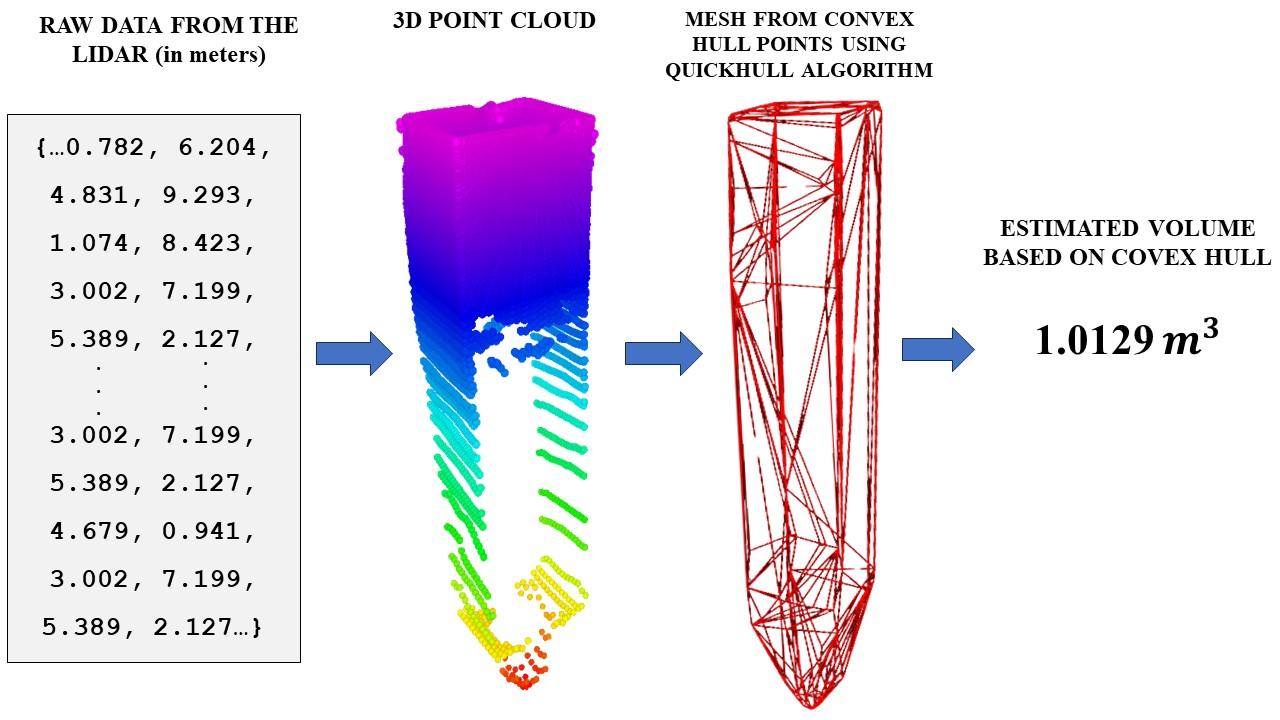
\includegraphics[width=0.9\textwidth]{Figures/volume-estimation-example}
	\caption{Example of the Volume Estimation Process of the System}
	\label{ch4:fig:volume-estimation-example}
\end{figure}

\section{Web Application Implementation}
The implementation result of the analysis for developing the web application is discussed in this section.

%\subsection{UI Dashboard Section}
% \subsubsection*{Main Dashboard Section}
The developed main dashboard of the UI, as shown in Figure \ref{ch4:fig:main-dashboard}, consists of three distinct sections. On the left side is the System Status section provides visual feedback regarding the establishment of the connection with the system, allowing users to monitor and verify the connection status. Additionally, users can access a list of currently active topics by clicking the List of Topics button. In the center section, users can visualize with the 3D point cloud data scanned from the system. This includes functionalities such as zooming in and out or moving the visualization. Moreover, in this section the start and stop scanning button is located, enabling users to send command to the system. Finally, on the right side, users can access volume measurement values and other numerical information, such as storage capacity. Users also have the option to input the known maximum volume capacity of the storage bin being used. The save button is also located in this section to store in the database the Empty Space Volume, Product Volume and the Percentage Capacity of the storage bin. \\

\begin{figure}[H]
	\centering
	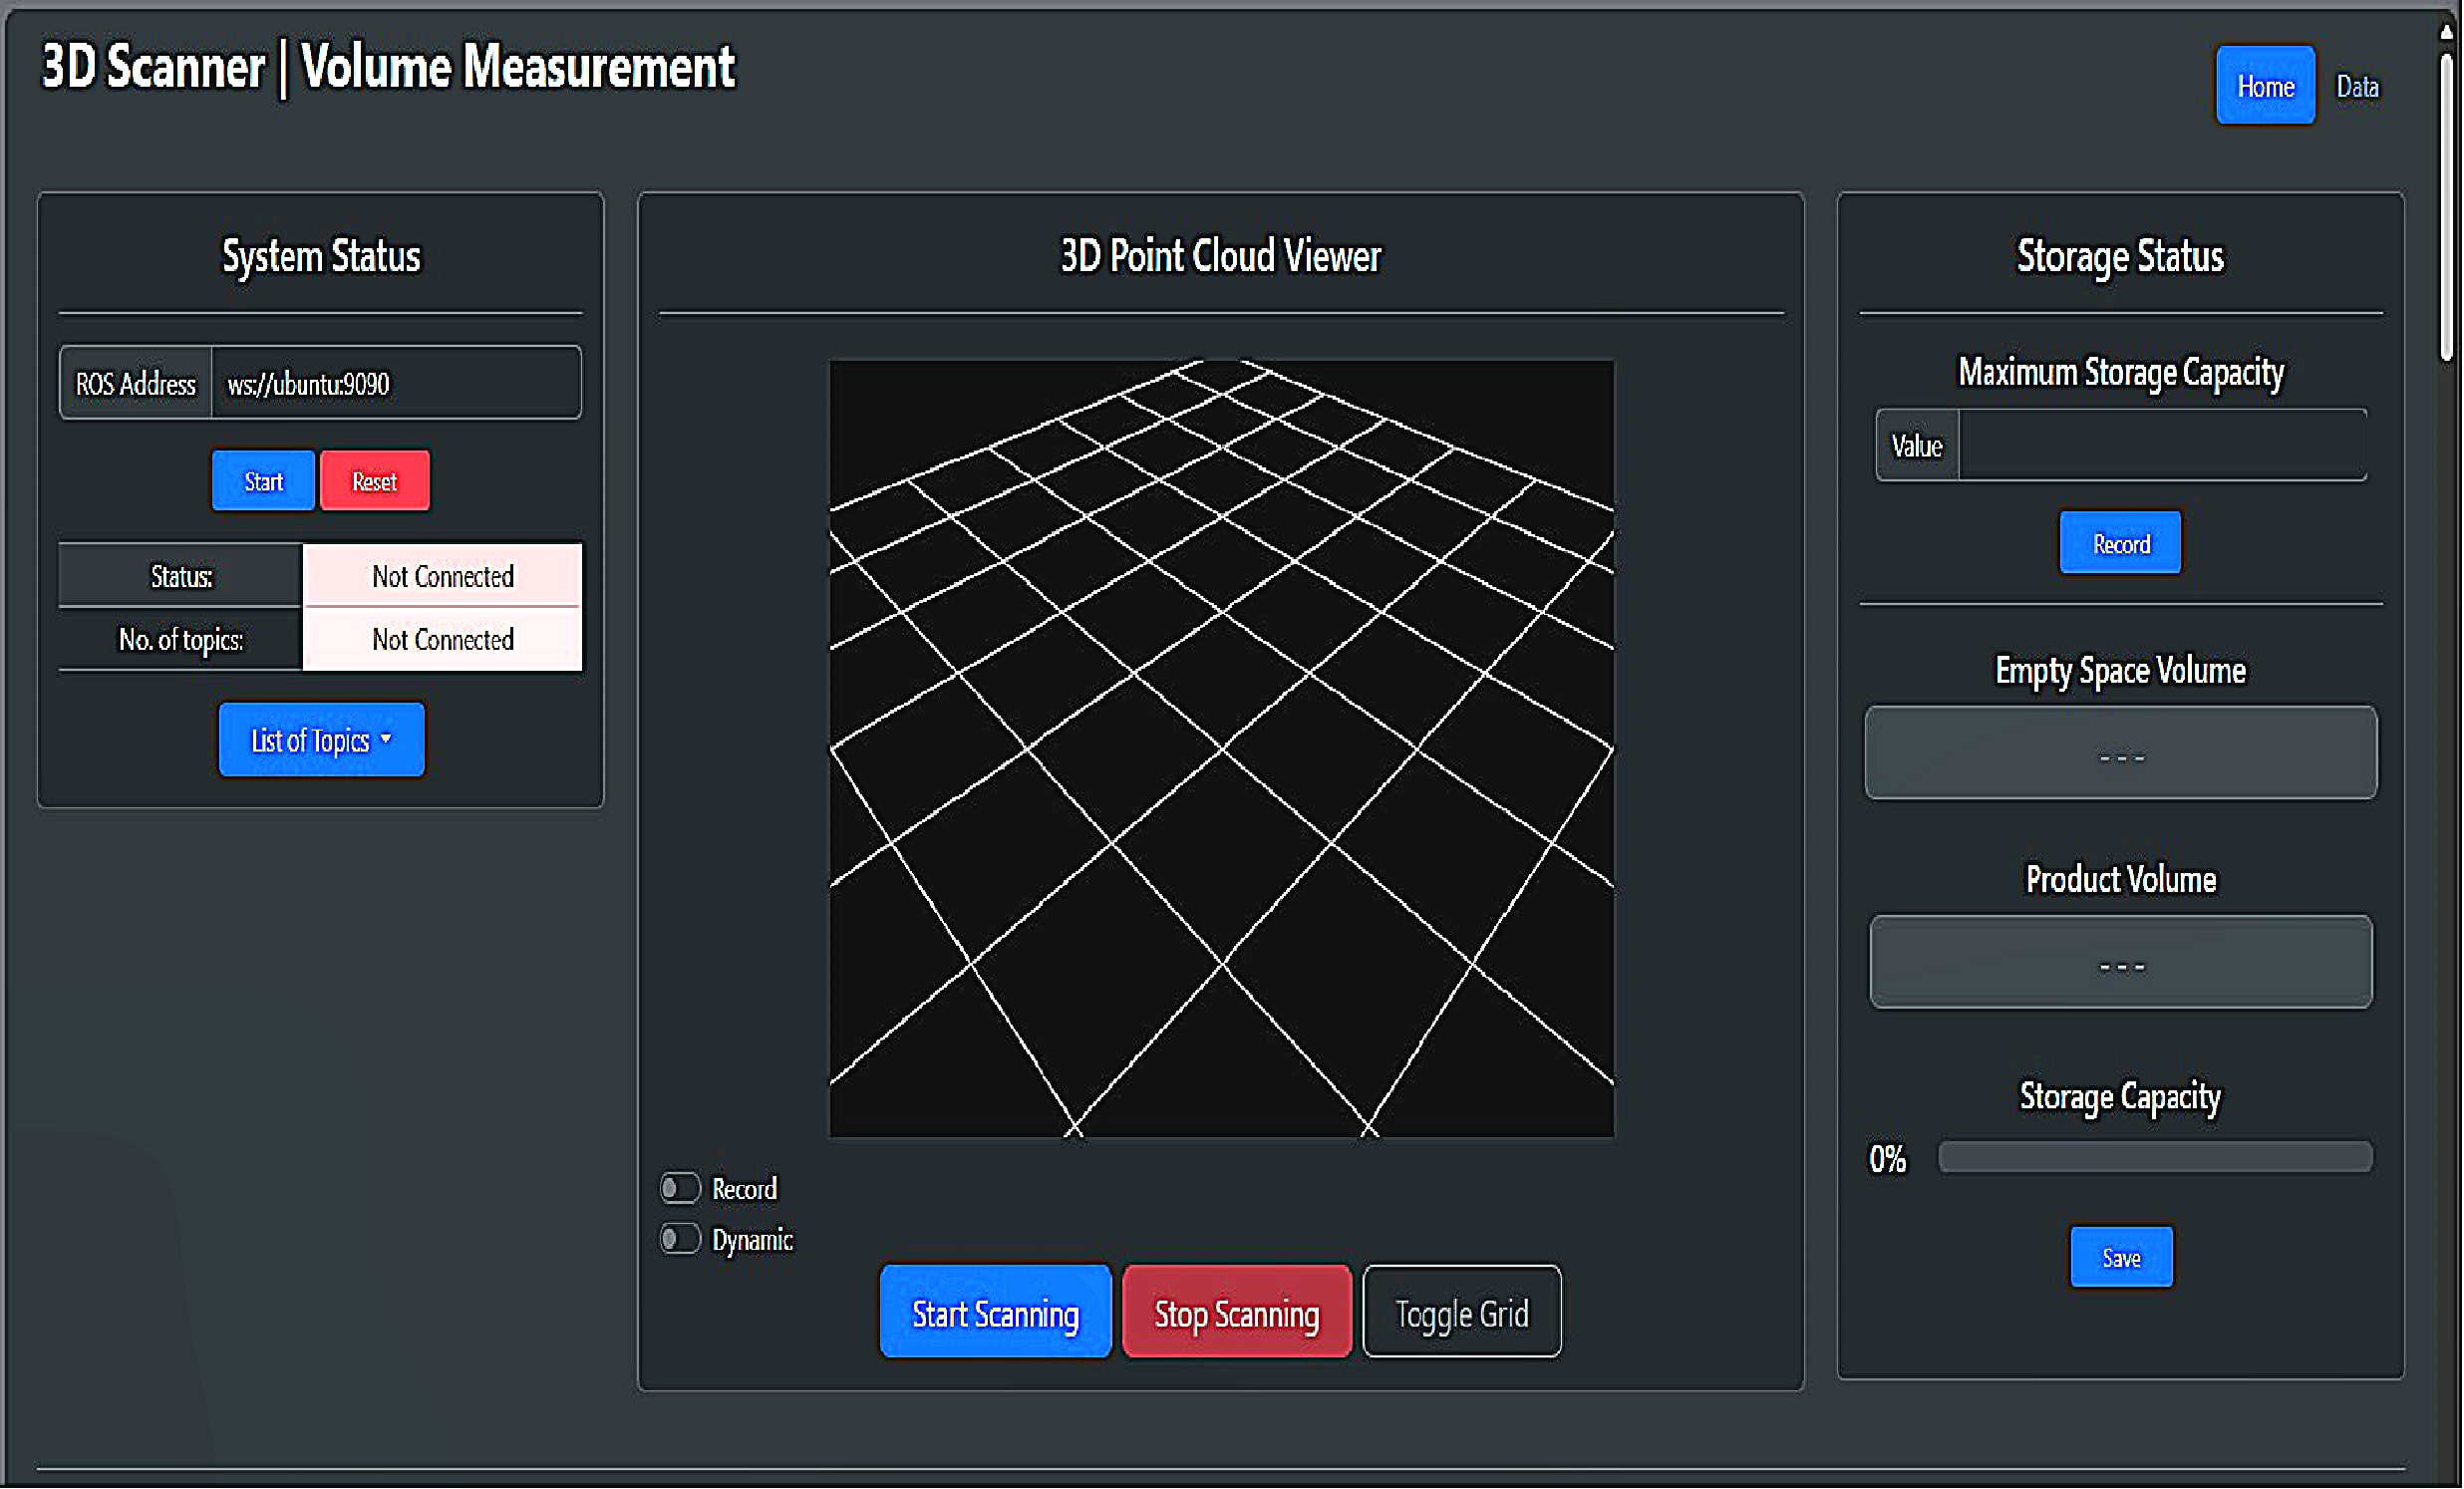
\includegraphics[width=1\textwidth]{Figures/main-dashboard-resize-phone}
	\caption{Main Dashboard}
	\label{ch4:fig:main-dashboard}
\end{figure}

% \subsubsection*{Data Section}

In the data section of the dashboard, users can visualize both the data table and the graph, as depicted in figures \ref{ch4:fig:data-section}, respectively. This data was retrieved from the developed database that were running locally. \\
\begin{figure}[H]
	\centering
	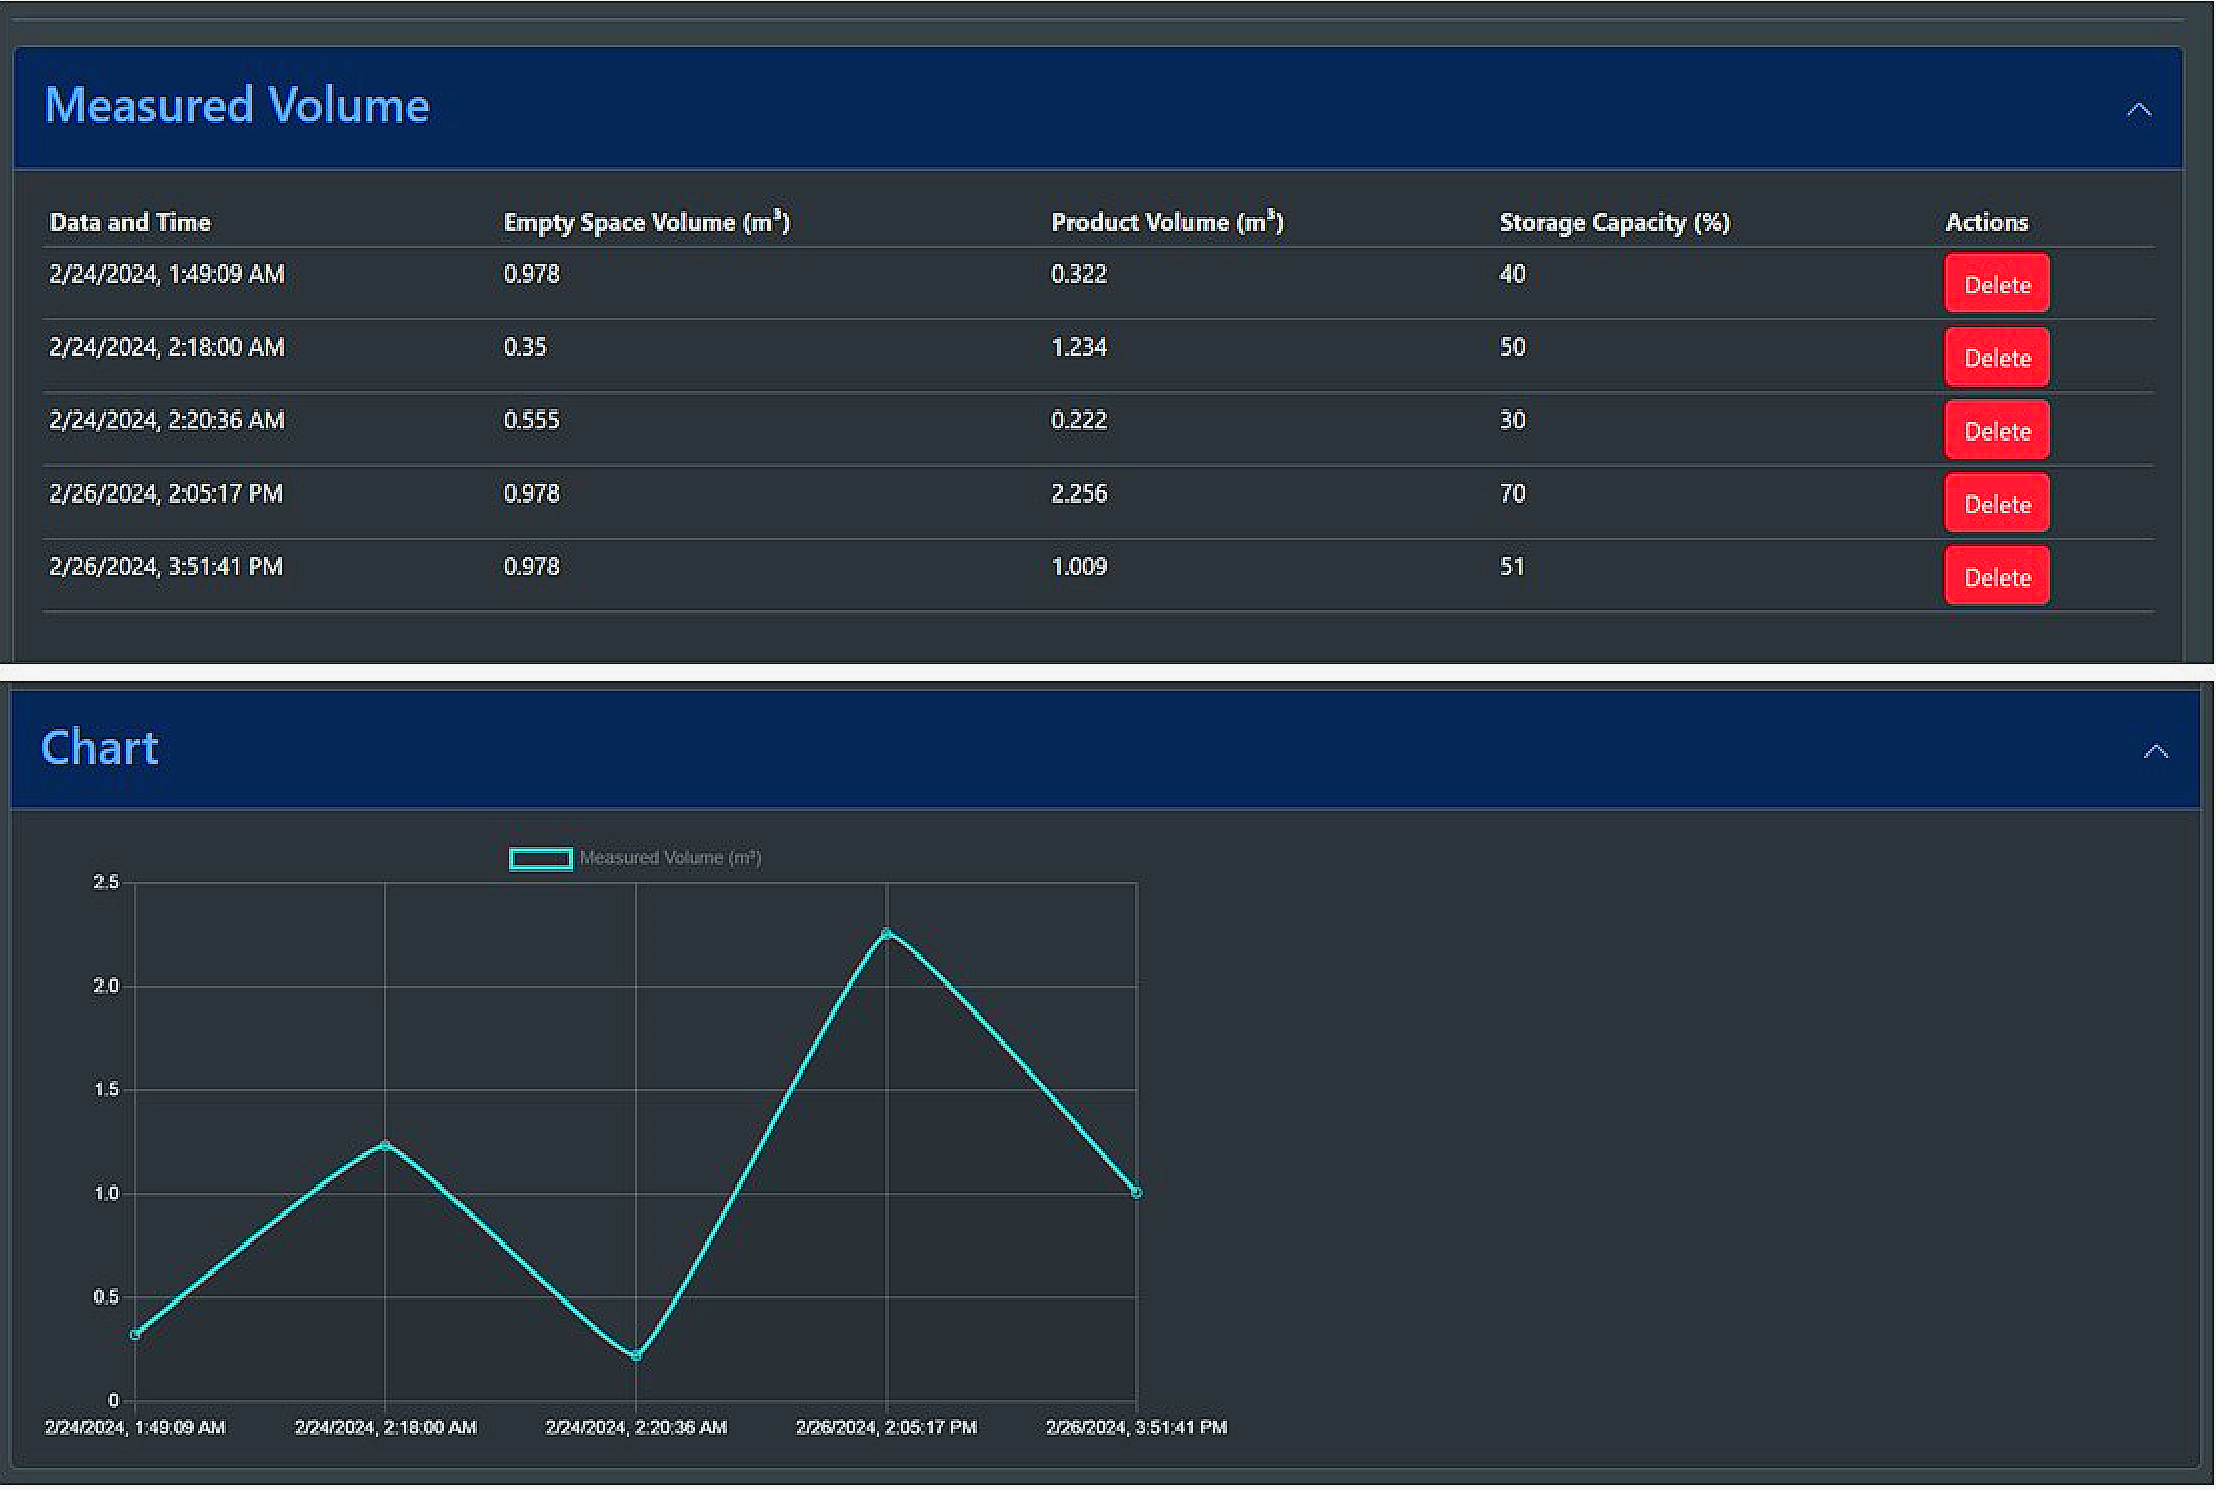
\includegraphics[width=1\textwidth]{Figures/data-section-resize-phone}
	\caption{Data Section}
	\label{ch4:fig:data-section}
\end{figure}

%\subsection{Database Integration}
The developed database was integrated to the web application, this database was running locally. Figure \ref{ch4:fig:database-schema-design} shows the single database table schema. The table shows a unique identifier for each record (id), a date and time stamp (date), and flout values for the empty space (empty\_space\_volume), product volume (product\_volume) and int value for storage capacity (storage\_capacity).

\begin{figure}[H]
	\centering
	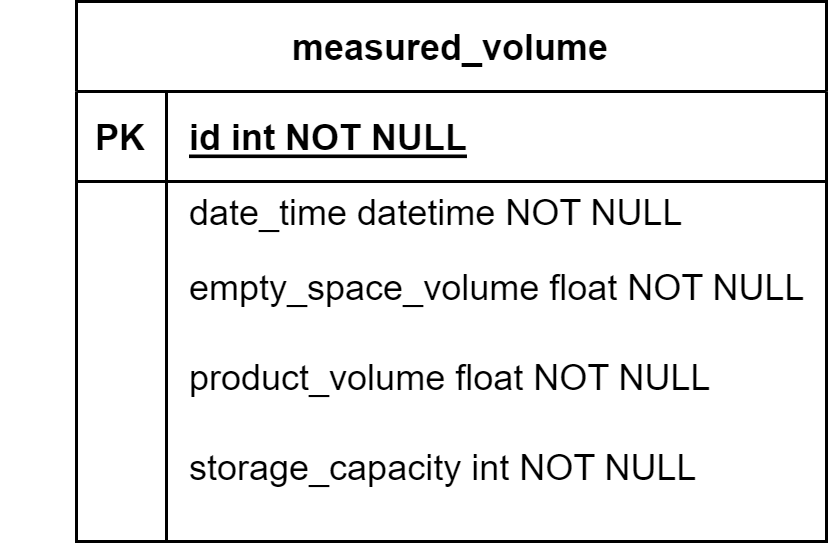
\includegraphics[width=0.5\textwidth]{Figures/database-schema-design}
	\caption{Single Database Schema of the Web Application}
	\label{ch4:fig:database-schema-design}
\end{figure}

\subsection{Overall System Integration}
The system and the Web interface were integrated and test their functionalities. The connection between the system and the web application were verified. Both system are within the same local network and utilizes WebSocket communication protocol, this protocol were discussed in the section \ref{ch3:subsec:overall-system-integration}. After verifying the connection between the systems, further tests were conducted to ensure successful overall system integration.
\section{System Testing and Evaluation Result}

After conducting the various tests outlined in Section \ref{ch3:sec:TestingAndEvaluation}, the following result of each testing  is discussed and evaluate in this section.

\subsection{LiDAR and Servo Calibration Test Result}
This section discusses the results of the calibration tests conducted to fine-tune the range measurement capabilities of the LiDAR sensor and the rotational accuracy of the servo motor. The actual images of the calibration testing is shown in Appendix \ref{appen:b}.
\subsubsection{LiDAR Range Calibration}
Five trials were conducted, with the LiDAR sensor capturing range data for five different reference points. The results of the calibration test are summarized in Table \ref{table:lidar_range_calibration}. \\

\begin{table}[H]
	\centering
	\begin{threeparttable}
		\fullwidthcaption{LiDAR Range Calibration Results}
		\label{table:lidar_range_calibration}
		\begin{tabular}{l c c c c c r}
			\toprule
			\textbf{\thead{Actual                                                                                        \\ Range (m)}} & \multicolumn{5}{c}{\textbf{Measured Range (m)}} & \textbf{Average (m)}                                                                    \\
			{}  & \textbf{Trial 1} & \textbf{Trial 2} & \textbf{Trial 3} & \textbf{Trial 4} & \textbf{Trial 5} &         \\ \midrule
			1   & 1.0134           & 1.0135           & 1.0367           & 1.0154           & 1.0135           & 1.0185  \\
			1.5 & 1.5267           & 1.5278           & 1.5165           & 1.5073           & 1.4975           & 1.51516 \\
			2   & 2.0289           & 2.0353           & 2.0145           & 2.0184           & 2.0095           & 2.02132 \\
			2.5 & 2.5241           & 2.5342           & 2.5092           & 2.5276           & 2.5502           & 2.52906 \\
			3   & 3.0412           & 3.0353           & 3.0452           & 3.0221           & 3.0317           & 3.0351  \\ \bottomrule
		\end{tabular}
	\end{threeparttable}
\end{table}

\subsubsection{Servo Angle Calibration}
The servo angle calibration test focused on assessing the rotational accuracy of the servo motor, which determines the orientation of the LiDAR sensor during scanning operations. Similar to the LiDAR range calibration, five trials were conducted to evaluate the servo's performance across various angular positions. The results of the calibration test are presented in Table \ref{table:servo-angle-calibration-result}. \\

\begin{table}[H]
	\centering
	\begin{threeparttable}
		\fullwidthcaption{Sevo Angle Calibration Results}
		\label{table:servo-angle-calibration-result}
		\begin{tabular}{l c c c c c r}
			\toprule
			\textbf{\thead{Actual                                                                                      \\ Angle ($^{\circ}$)}} & \multicolumn{5}{c}{\textbf{Measured Angle ($^{\circ}$)}} & \textbf{Average ($^{\circ}$)}                                                                    \\
			{}  & \textbf{Trial 1} & \textbf{Trial 2} & \textbf{Trial 3} & \textbf{Trial 4} & \textbf{Trial 5} &       \\ \midrule
			35  & 35               & 36               & 35               & 35               & 35               & 35.2  \\
			70  & 70               & 71               & 70               & 70               & 69               & 70    \\
			105 & 106              & 105              & 106              & 104              & 105              & 105.2 \\
			140 & 140              & 141              & 139              & 141              & 140              & 140.2 \\
			175 & 175              & 175              & 174              & 174              & 176              & 174.8 \\ \bottomrule
		\end{tabular}
	\end{threeparttable}
\end{table}

\subsection{System Volume Measurement Calibration Result}
The different volume measurement calibration testing outline in section \ref{ch3:subsection:volume-measurement-test} were conducted. The results of these testing are discussed further in this section, and the images of the actual testing conducted is shown in appendix \ref{appen:b}.
\subsubsection{Testing Setup Result}

The design specifications outlined of the proposed storage bin in section \ref{ch3:subsubsec:testing-setup} were implemented to construct a mock-up storage bin. In the actual mock-up bin consists of three distinct geometric shapes as depicted in Figure \ref{ch4:fig:constructed-storage-bin}. The dimensions of each shape were manually measured using a steel tape measure.

\begin{itemize}
	\item The rectangular shape has the following dimension:
	      \begin{itemize}
		      \item Height: 2.775 meters
		      \item Length: 0.5 meters
		      \item Width: 0.69 meters
	      \end{itemize}
	\item The pyramidal frustum shape has the following dimensions:
	      \begin{itemize}
		      \item Upper length: 0.5 meters
		      \item Upper width: 0.69 meters
		      \item Height: 0.03 meters
		      \item Lower length and width: 0.42 meters
	      \end{itemize}
	\item The conical frustum shape features the following dimensions:
	      \begin{itemize}
		      \item Top radius: 0.21 meters
		      \item Bottom radius: 0.17 meters
		      \item Height: 0.42 meters
	      \end{itemize}
\end{itemize}

With these dimensions, the individual and total volume capacities of the storage bin were calculated. Table \ref{ch4:tab:volume-calculation} provides a summary of the measured individual and total volume capacity of the bin. \\


\begin{table}[H]
	\centering
	\smalltable{Individual and Total Volume of the Storage Bin}
	\label{ch4:tab:volume-calculation}
	\begin{tabularx}{0.69\textwidth}{l c c c r}
		\toprule
		\textbf{Shape}    & {} & {} & {} & \textbf{Actual Volume ($m^{3}$)} \\ \midrule

		Rectangular       & {} & {} & {} & 0.9573                           \\

		Pyramidal Frustum & {} & {} & {} & 0.0077                           \\

		Conical Frustum   & {} & {} & {} & 0.0478088                        \\ \midrule

		Total             & {} & {} & {} & 1.012875                         \\ \bottomrule
	\end{tabularx}
\end{table}

\begin{figure}[H]
	\centering
	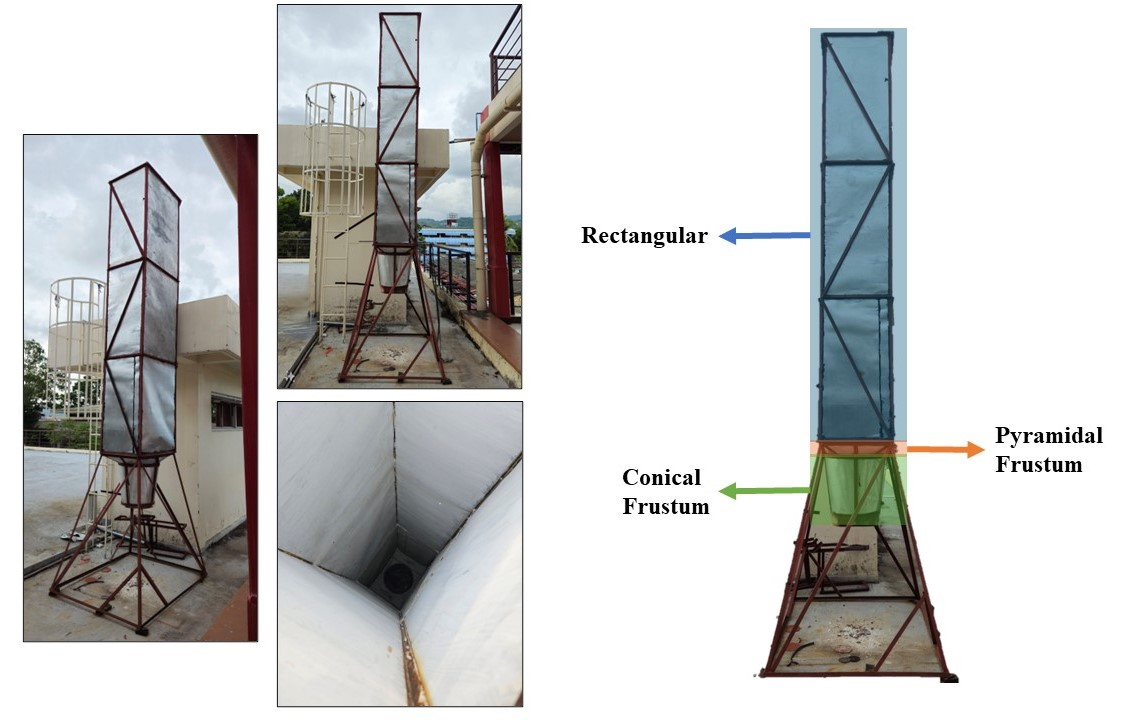
\includegraphics[width=0.9\textwidth]{Figures/constructed_storage_bin.jpg}
	\caption{Actual Flour Storage Bin Created}
	\label{ch4:fig:constructed-storage-bin}
\end{figure}

% \subsection{Created Mock-up Storage Bin}
% The design specifications outlined of the proposed storage bin in section \ref{ch3:subsec:testing-setup} were implemented to construct a mock-up storage bin. In the actual mock-up bin consists of three distinct geometric shapes as depicted in Figure \ref{ch4:fig:constructed-storage-bin}. The dimensions of each shape were manually measured using a steel tape measure.

% The rectangular shape of the bin measures 2.775 meters in height, with lengths and widths of 0.5 and 0.69 meters respectively. The pyramidal frustum shape has an upper length and width of 0.5 and 0.69 meters respectively, with a height of 0.03 meters, and a lower length and width of 0.42 meters. Lastly, the conical frustum shape features a top radius of 0.21 meters, a bottom radius of 0.17 meters, and a height of 0.42 meters.

% With these dimensions, the individual and total volume capacities of the storage bin were calculated. Table \ref{ch4:tab:volume-calculation} provides a summary of the measured individual and total volume capacity of the bin. \\


% \begin{table}[H]
% 	\centering
% 	\caption{Individual and Total Volume of the Storage Bin}
% 	\label{ch4:tab:volume-calculation}
% 	\begin{tabular}{l r}
% 		\toprule
% 		\textbf{Shape}    & \textbf{Actual Volume ($m^{3}$)} \\ \midrule

% 		Rectangular       & 0.9573                           \\

% 		Pyramidal Frustum & 0.0077                           \\

% 		Conical Frustum   & 0.0478088                        \\ \midrule

% 		Total             & 1.012875                         \\ \bottomrule
% 	\end{tabular}
% \end{table}

% \begin{figure}[H]
% 	\centering
% 	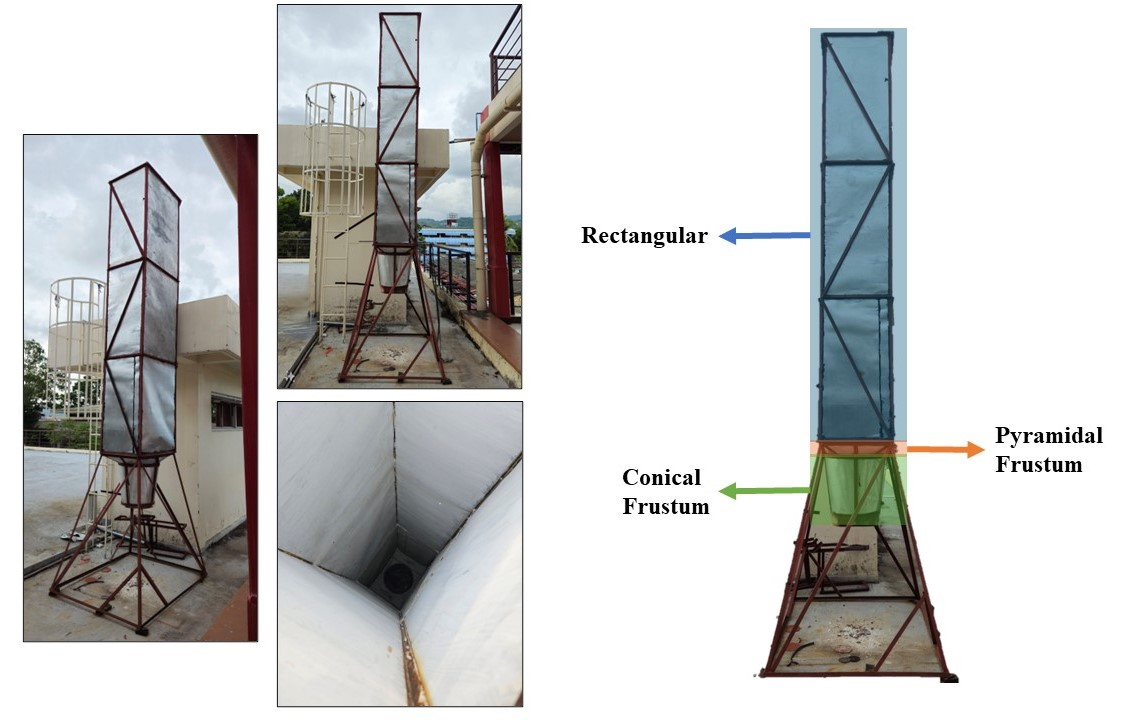
\includegraphics[width=0.9\textwidth]{Figures/constructed_storage_bin.jpg}
% 	\caption{Constructed Storage Bin Setup}
% 	\label{ch4:fig:constructed-storage-bin}
% \end{figure}

% \subsection{Actual System Setup}

The actual field system setup shown in figure \ref{ch4:fig:actual-system-setup} demonstrate the placement of the 3D Point Cloud Scanner System and the end-user device where the web application is running. The actual field of testing situated within the university premises. \\

\begin{figure}[H]
	\centering
	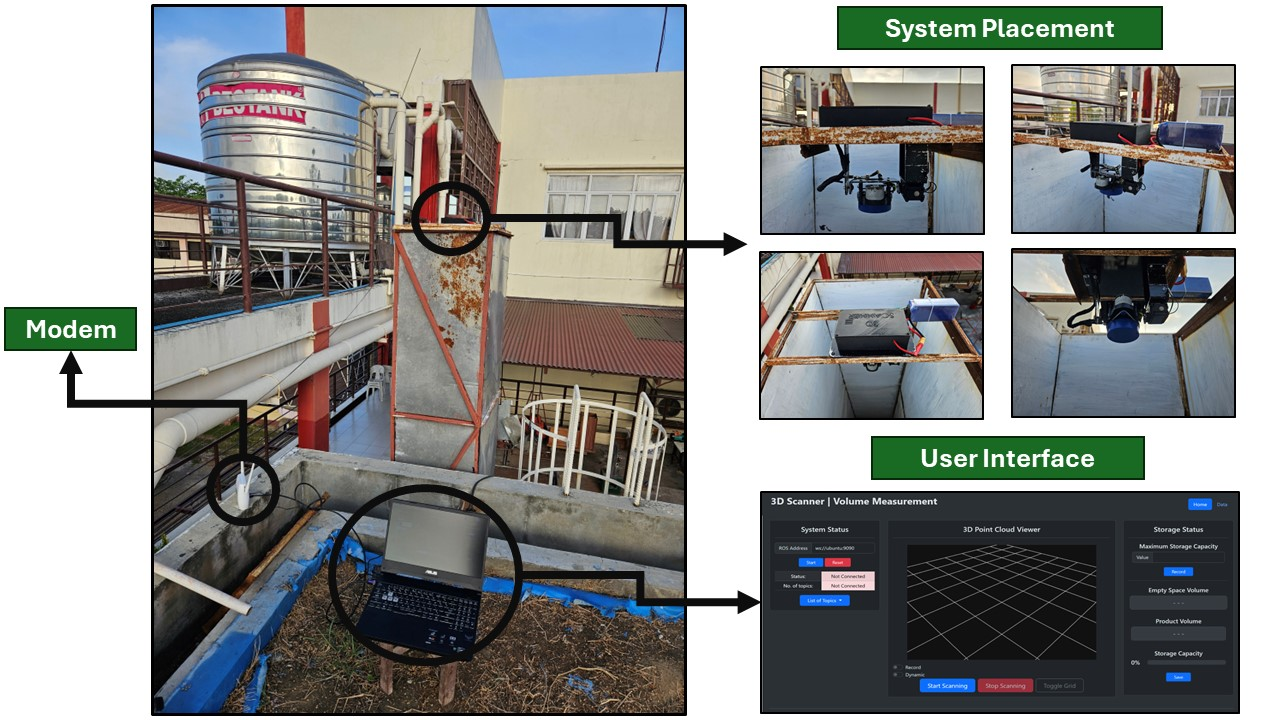
\includegraphics[width=1\textwidth]{Figures/actual-system-setup}
	\caption{Testing Field and The Actual System Setup}
	\label{ch4:fig:actual-system-setup}
\end{figure}

\subsubsection{Empty Storage Volume Measurement Calibration Test Result}
Multiple scans and volume measurement of an empty storage bin were performed. Figure \ref{ch4:fig:empty-bin-point-cloud} shows the the sample point cloud scan of the system and the actual empty bin. Table \ref{table:test_case_1_results} presents the results obtained from 37 scanning trials. The actual visualization of the point cloud and volume are shown in figure \ref{ch4:fig:web-point-cloud-and-volume}. \\

\begin{figure}[H]
	\centering
	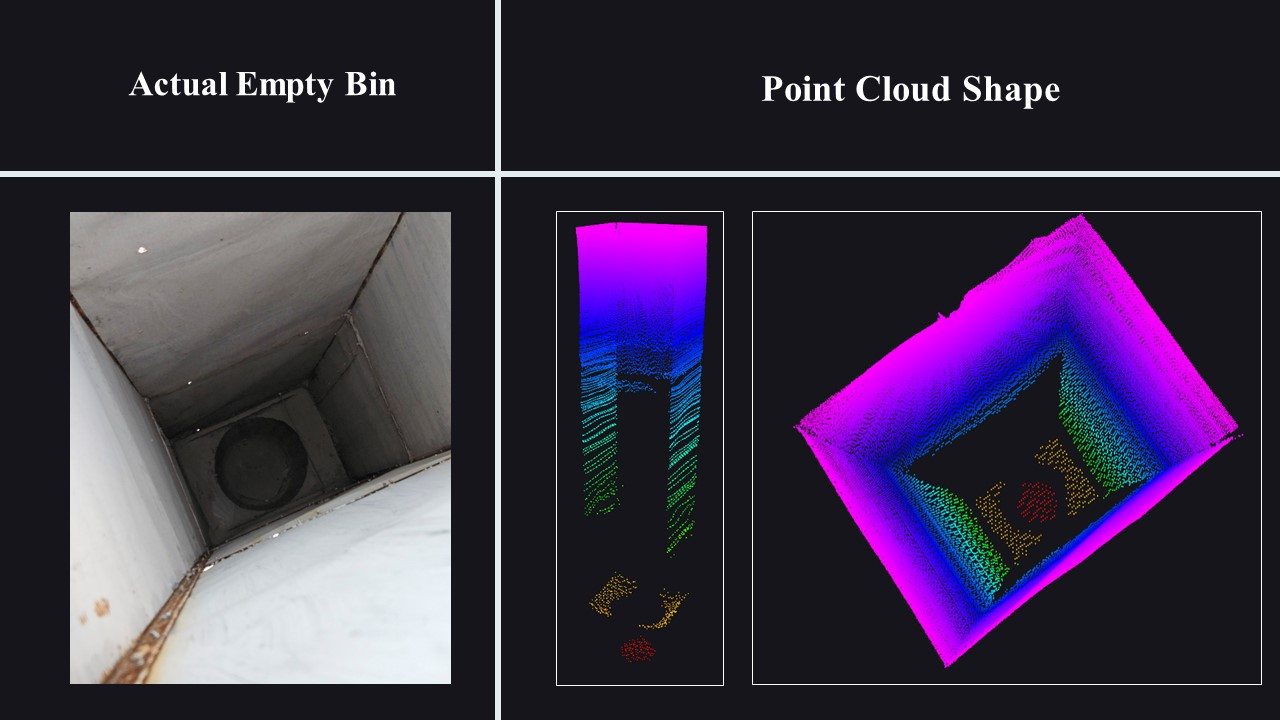
\includegraphics[width=1\textwidth]{Figures/empty-bin-point-cloud}
	\caption{Actual Empty Bin and Scanned Point Cloud Data}
	\label{ch4:fig:empty-bin-point-cloud}
\end{figure}

\begin{figure}[H]
	\centering
	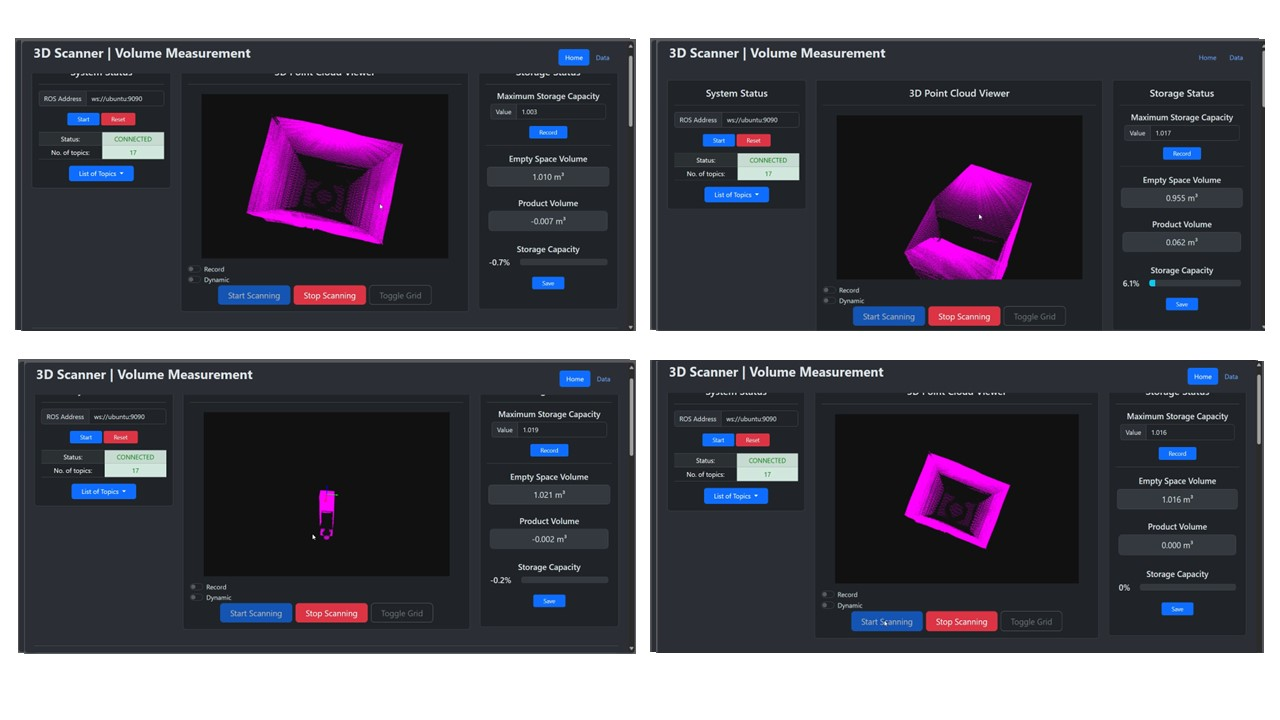
\includegraphics[width=1\textwidth]{Figures/web-point-cloud-and-volume-1}
	\caption{Actual Web Visualization of Point Cloud and Volume}
	\label{ch4:fig:web-point-cloud-and-volume}
\end{figure}

\begin{table}[H]
	\centering
	\begin{threeparttable}
		\fullwidthcaption{Actual and Measured Volume of Empty Storage Bin Volume Measurement Result}
		\label{table:test_case_1_results}
		\begin{tabular}{l c r}
			\toprule
			\textbf{Trials} & \textbf{\thead{Measured Volume of the System ($m^{3}$)}} & \textbf{\thead{Storage Actuatl Total Volume ($m^{3}$)}} \\ \midrule

			1               & 1.0118                                                   & 1.0129                                                  \\
			2               & 1.0120                                                   & 1.0129                                                  \\
			3               & 1.0120                                                   & 1.0129                                                  \\
			4               & 1.0130                                                   & 1.0129                                                  \\
			5               & 1.0123                                                   & 1.0129                                                  \\
			6               & 1.0130                                                   & 1.0129                                                  \\
			7               & 1.0110                                                   & 1.0129                                                  \\
			8               & 1.0110                                                   & 1.0129                                                  \\
			9               & 1.0112                                                   & 1.0129                                                  \\
			10              & 1.0123                                                   & 1.0129                                                  \\
			11              & 1.0120                                                   & 1.0129                                                  \\
			12              & 1.0120                                                   & 1.0129                                                  \\
			13              & 1.0110                                                   & 1.0129                                                  \\
			14              & 1.0190                                                   & 1.0129                                                  \\
			15              & 1.0110                                                   & 1.0129                                                  \\
			16              & 1.0130                                                   & 1.0129                                                  \\
			17              & 1.0140                                                   & 1.0129                                                  \\
			18              & 1.0120                                                   & 1.0129                                                  \\
			19              & 1.0110                                                   & 1.0129                                                  \\
			20              & 1.0100                                                   & 1.0129                                                  \\
			21              & 1.0130                                                   & 1.0129                                                  \\
			22              & 1.0160                                                   & 1.0129                                                  \\
			23              & 1.0140                                                   & 1.0129                                                  \\
			24              & 1.0140                                                   & 1.0129                                                  \\
			25              & 1.0160                                                   & 1.0129                                                  \\
			26              & 1.0150                                                   & 1.0129                                                  \\
			27              & 1.0110                                                   & 1.0129                                                  \\
			28              & 1.0110                                                   & 1.0129                                                  \\
			29              & 1.0110                                                   & 1.0129                                                  \\
			30              & 1.0160                                                   & 1.0129                                                  \\
			31              & 1.0170                                                   & 1.0129                                                  \\
			32              & 1.0127                                                   & 1.0129                                                  \\
			33              & 1.0120                                                   & 1.0129                                                  \\
			34              & 1.0123                                                   & 1.0129                                                  \\
			35              & 1.0110                                                   & 1.0129                                                  \\
			36              & 1.0130                                                   & 1.0129                                                  \\
			37              & 1.0130                                                   & 1.0129                                                  \\ \bottomrule
		\end{tabular}
	\end{threeparttable}
\end{table}


% \begin{figure}[H]
% 	\centering
% 	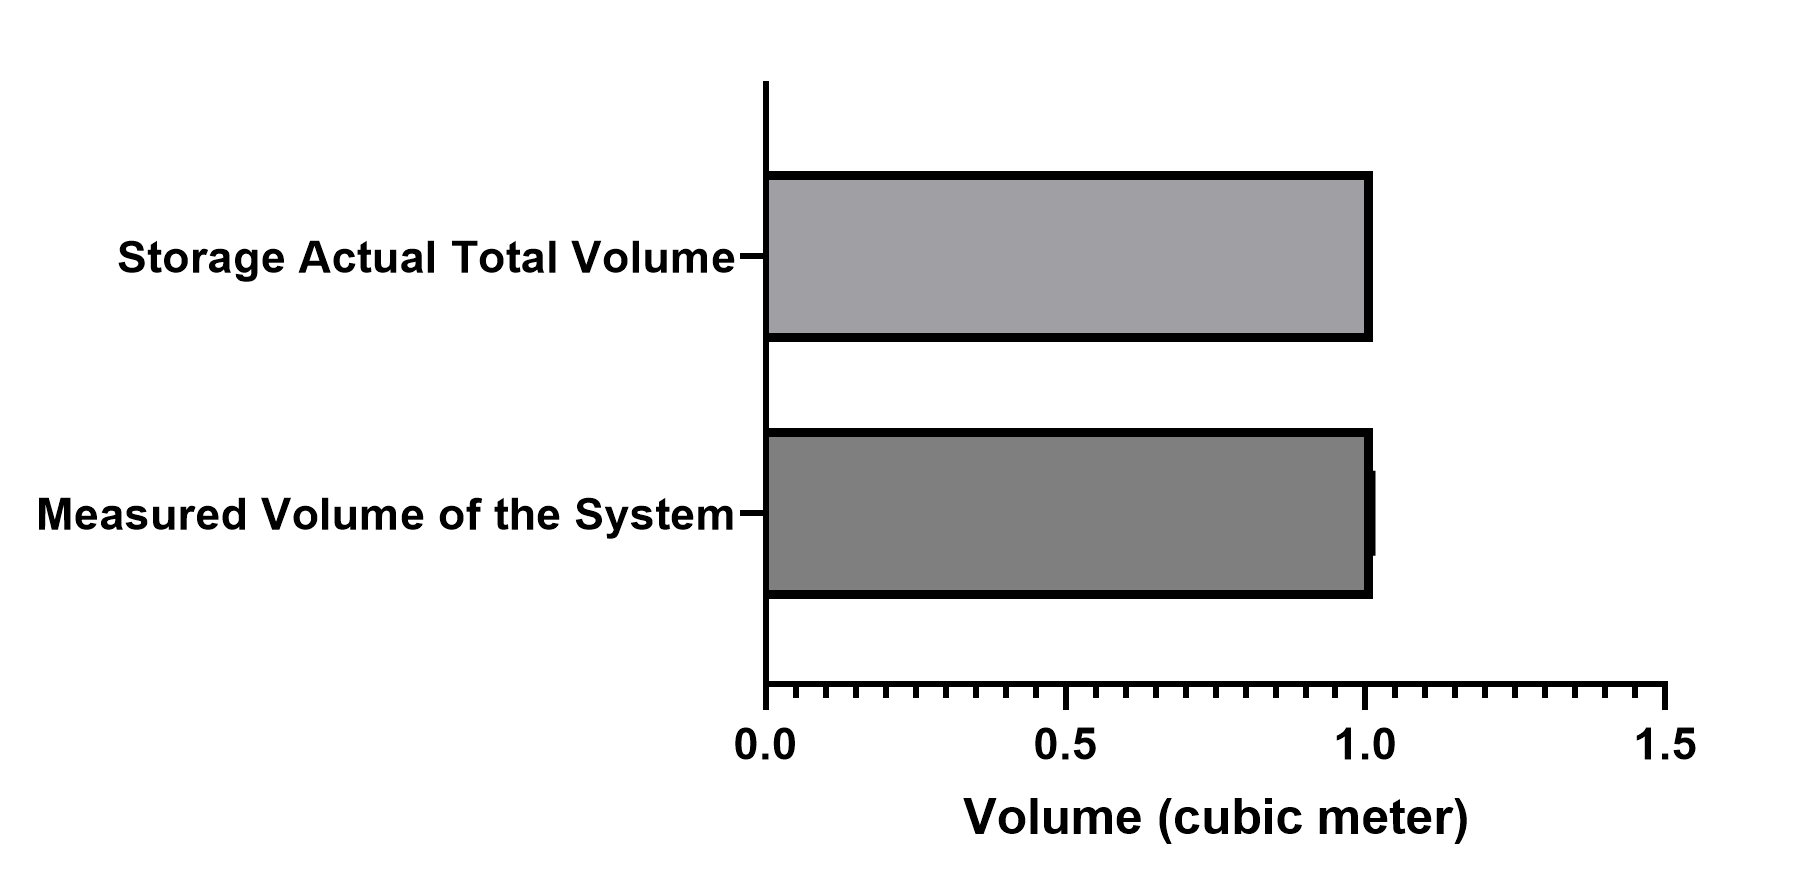
\includegraphics[width=0.8\textwidth]{Figures/test1_graph}
% 	\caption{Distribution of the Measurement of the System to the Actual Total Volume of the Storage}
% 	\label{ch4:fig:test-case-1-graph}
% \end{figure}

Based on the graph shown in figure \ref{ch4:fig:test-case-1-graph}, the average measured volume of the system is 1.0128 $m^3$. The actual total volume of the storage bin is 1.0129 $m^3$. To determine the actual volume of the storage bin, the study calculated the total volume it can store based on its dimensions and geometric volume.

To determine whether it is statistically different from the mean of the storage total volume of 1.0129 $m^3$ to the mean measured volume of the system, the study conducted a One-Sample t-test. According to the p.value which is above 0.05, there is no statistically significant difference detected.

% The average measured volume across all trials was determined to be 1.00919 $m^{3}$ and with an uncertainty of $\pm$ 0.0155 $m^{3}$. With a gathered Mean Absolute Percentage Error (MAPE) of 0.599377608 \%.
\subsubsection{Different Volume Quantity Measurement Calibration Test Result}

In this test, three different scenarios were conducted as discussed in section \ref{ch3:subsubsec:different-volume-measurement-test}, the flour storge bin was filled with different volume flour materials: \textbf{(1) 0.0594 $m^3$, (2) 0.4752 $m^3$ and (3) 0.7128 $m^3$}. A container with a known volume was used throughout this test for filling the storage bin as shown in figure \ref{ch4:fig:known-volume}. This container was measured manually and has a total volume capacity of 0.0594 $m^3$.\\

\begin{figure}[H]
	\centering
	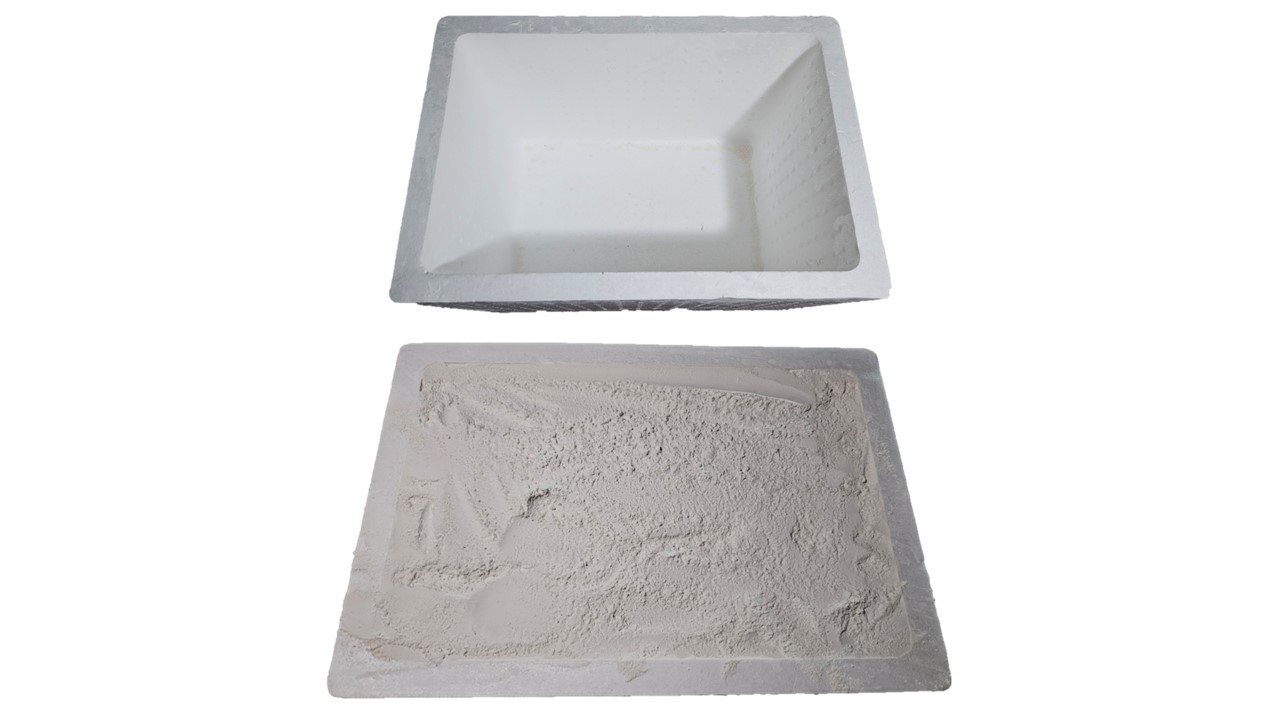
\includegraphics[width=0.8\textwidth]{Figures/known-volume}
	\caption{Container with a Known Volume Used for Testing}
	\label{ch4:fig:known-volume}
\end{figure}


% \subsubsection*{Test Case 2.1: Storage Bin Filled to 5.8\% of Maximum Capacity}

\begin{enumerate}
	\item \textbf{Storage Bin Filled with 0.0594 $m^3$ of Flour}

	      Figure \ref{ch4:fig:test_2-1_contours} illustrate the actual flour surface contours along with the point cloud shapes by the system. The measured volumes of the two contours and the distribution of the data is presents in table \ref{table:test_case_2-1_results}. % and figure \ref{ch4:fig:test-case-2-1-graph} respectively. \\
	      \\
	      \begin{figure}[H]
		      \centering
		      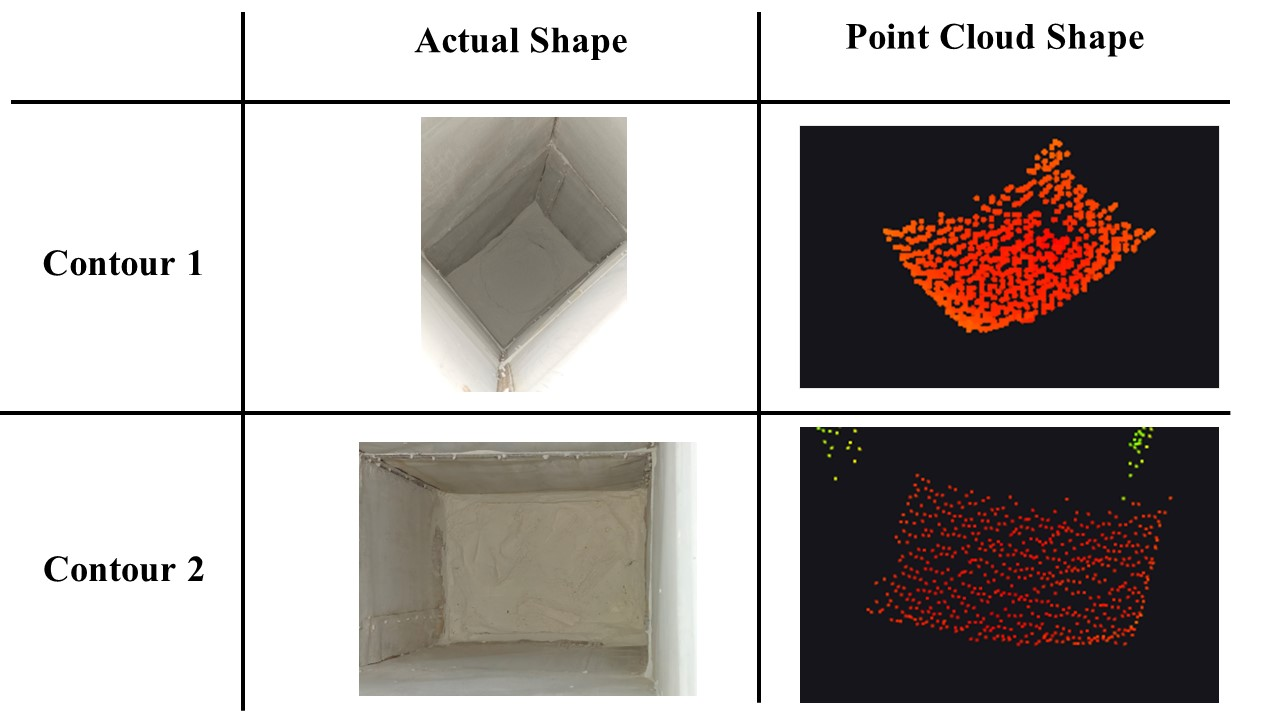
\includegraphics[width=0.8\textwidth]{Figures/test_2-1_contours}
		      \caption{Actual and Point Cloud Surface Contour of Test 1}
		      \label{ch4:fig:test_2-1_contours}
	      \end{figure}

	      Table \ref{table:test_case_2-1_results} presents the calibration result of the volume measurement of the system, which compares the measured volumes of two contours against a known volume of 0.0594 m³ across five trials. Contour 1 exhibited an average measured volume of 0.059678 m³, resulting in a slightly higher estimation of the actual volume. Conversely, Contour 2 demonstrated a closer correspondence with the known volume, with an average measurement of 0.0595 m³. Both contours displayed minimal deviations in measured volume across trials, suggesting reasonable accuracy and precision. \\

	      \begin{table}[H]
		      \centering
		      \begin{threeparttable}
			      \caption{Volume Measurements Calibration Result of the System Across Two Contours with A Known Volume of 0.0594 $m^3$}
			      \label{table:test_case_2-1_results}
			      \begin{tabular}{l c c r}
				      \toprule
				      \textbf{Trials} & \multicolumn{2}{c}{\textbf{Measured Volume ($m^{3}$)}} & \textbf{Known Volume} ($m^{3}$)          \\
				      {}              & Contour 1                                              & Contour 2                       & {}     \\ \midrule
				      1               & 0.06                                                   & 0.0592                          & 0.0594 \\
				      2               & 0.05934                                                & 0.0601                          & 0.0594 \\
				      3               & 0.058943                                               & 0.0589                          & 0.0594 \\
				      4               & 0.05976                                                & 0.0591                          & 0.0594 \\
				      5               & 0.059678                                               & 0.0602                          & 0.0594 \\ \midrule
				      Average         & 0.059678                                               & 0.0595                          & {}     \\ \bottomrule
			      \end{tabular}
		      \end{threeparttable}
	      \end{table}

	      %   \begin{figure}[H]
	      %       \centering
	      %       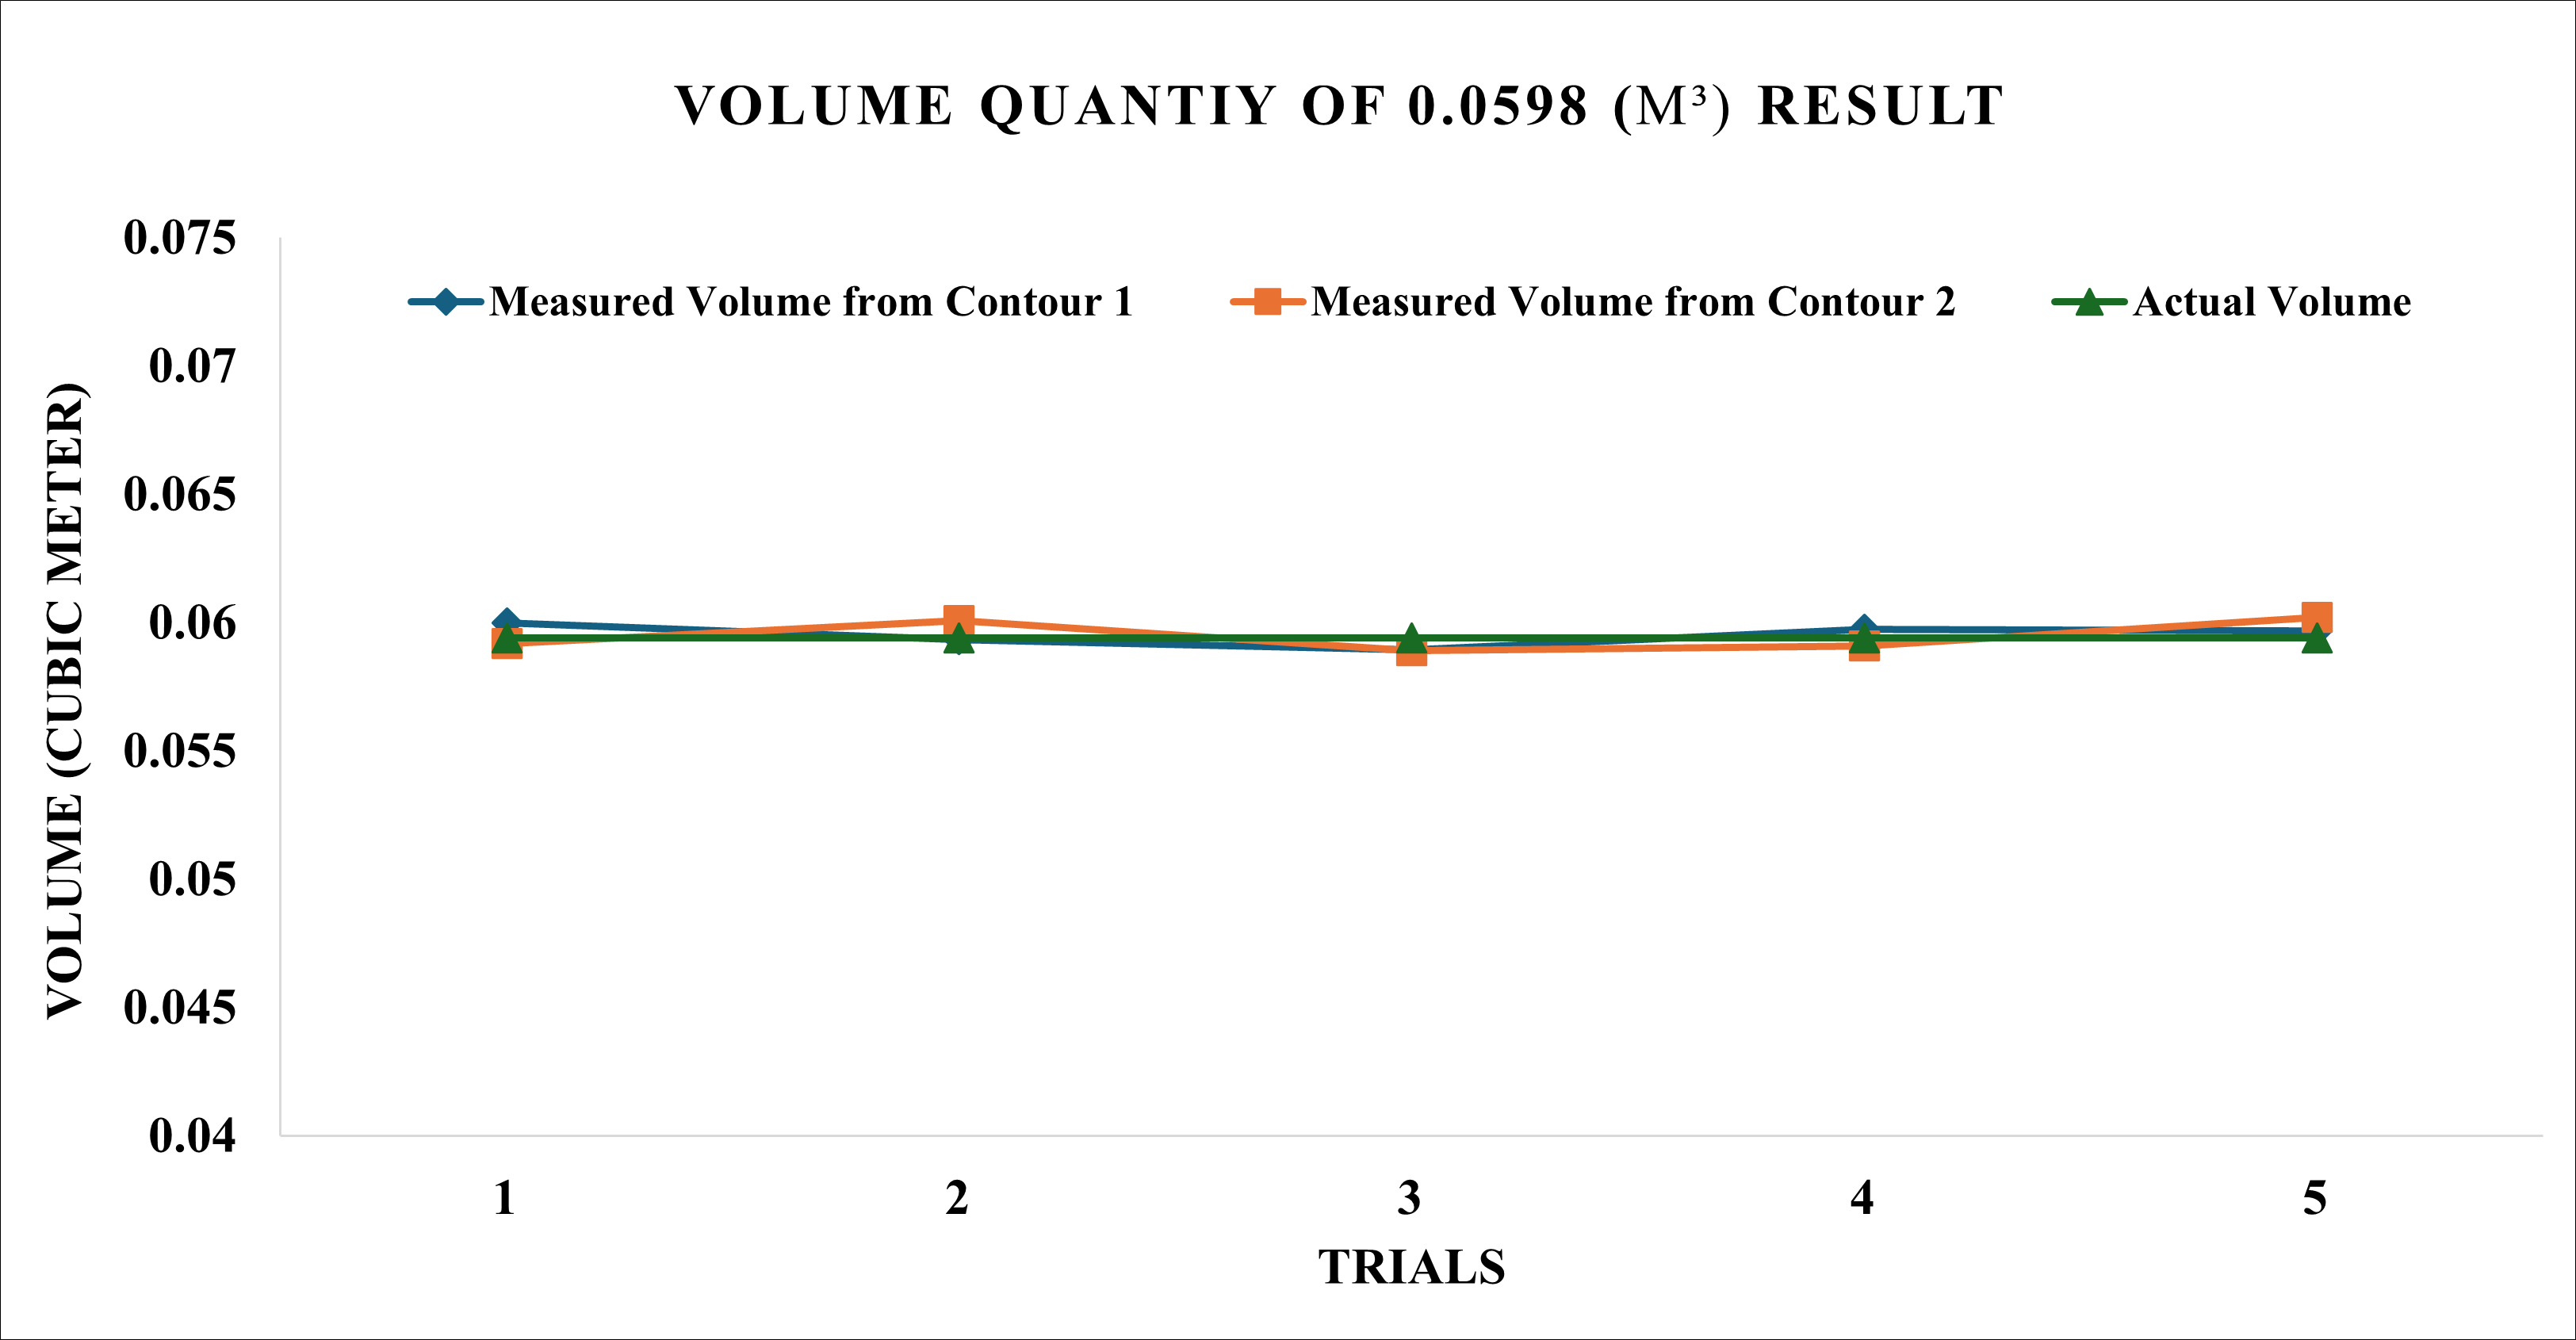
\includegraphics[width=0.8\textwidth]{Figures/test-case-2-1-graph}
	      %       \caption{Distribution of the Measured Volumes of two Contours}
	      %       \label{ch4:fig:test-case-2-1-graph}
	      %   \end{figure}

	      Based on the conducted ANOVA test and the statistic analysis table can be seen in Appendix \ref{appen:c} table \ref{table-anova-1}, there is no statistical difference for the 0.0594 $m^3$ level volume measurement according to the actual volume and those with different contours measured by the system with p value greater that 0.05.



	      %The results from test 1 gathered an average measured volume of 0.059678 $m^{3}$ and 0.0595 $m^{3}$ and a deviation of 0.00036 $m^{3}$ and 0.00054 $m^{3}$ from contour 1 and 2 respectively. Contour 1 achieved a MAPE of 0.591\%, while the contour 2 have a MAPE of 0.8417\%. Overall, test 1 gathered an average measured volume with uncertainty of 0.0595221 $\pm$ 0.00065 $m^{3}$ and an average MAPE of 0.7163\%. \\

	\item \textbf{Storage Bin Filled with 0.4752 $m^3$ of Flour}

	      A flour of 0.4752 $m^3$ was filled in the storage bin. Figure \ref{ch4:fig:test_2-2_contours} illustrates the actual flour surface contours along with the scanned point cloud contour by the system. The measured volumes across the two contours and the distribution of the data are presented in table \ref{table:test_case_2-2_results}. % and figure \ref{ch4:fig:test-case-2-2-graph}.
	      \\
	      \begin{figure}[H]
		      \centering
		      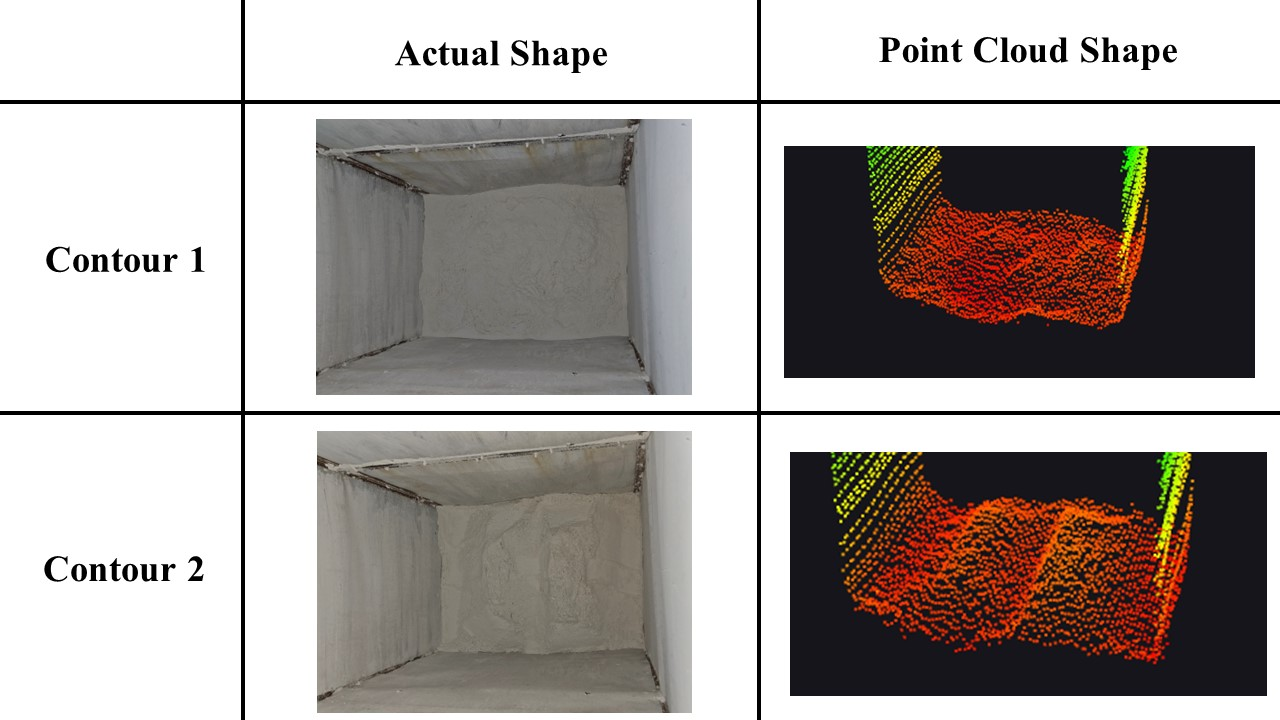
\includegraphics[width=0.8\textwidth]{Figures/test_2-2_contours}
		      \caption{Actual and Point Cloud Surface Contours of Test 2}
		      \label{ch4:fig:test_2-2_contours}
	      \end{figure}

	      The table \ref{table:test_case_2-2_results} presents the results of volume measurements calibration for a system across two contours, compared against a known volume of 0.4752 m³. Over five trials, Contour 1's measured volumes range from 0.470279 m³ to 0.4805594 m³, with an average of 0.47407038 m³, slightly lower estimation to the actual volume. Contour 2's measurements range from 0.464461 m³ to 0.485587 m³, with an average of 0.473391 m³, also slightly underestimating the actual volume. Both contours show minor variations, with Contour 1 being marginally closer to the actual volume on average. \\

	      \begin{table}[H]
		      \centering
		      \begin{threeparttable}
			      \caption{Volume Measurements Calibration Result of the System Across Two Contours with A Known Volume of 0.4752 $m^3$}
			      \label{table:test_case_2-2_results}
			      \begin{tabular}{l c c r}
				      \toprule
				      \textbf{Trials} & \multicolumn{2}{c}{\textbf{Measured Volume ($m^{3}$)}} & \textbf{Known Volume} ($m^{3}$)          \\
				      {}              & Contour 1                                              & Contour 2                       & {}     \\ \midrule
				      1               & 0.470418                                               & 0.472914                        & 0.4752 \\
				      2               & 0.470279                                               & 0.464461                        & 0.4752 \\
				      3               & 0.472061                                               & 0.473782                        & 0.4752 \\
				      4               & 0.4805594                                              & 0.485587                        & 0.4752 \\
				      5               & 0.4770345                                              & 0.470211                        & 0.4752 \\ \midrule
				      Average         & 0.47407038                                             & 0.473391                        & {}     \\ \bottomrule
			      \end{tabular}
		      \end{threeparttable}
	      \end{table}

	      %   \begin{figure}[H]
	      %       \centering
	      %       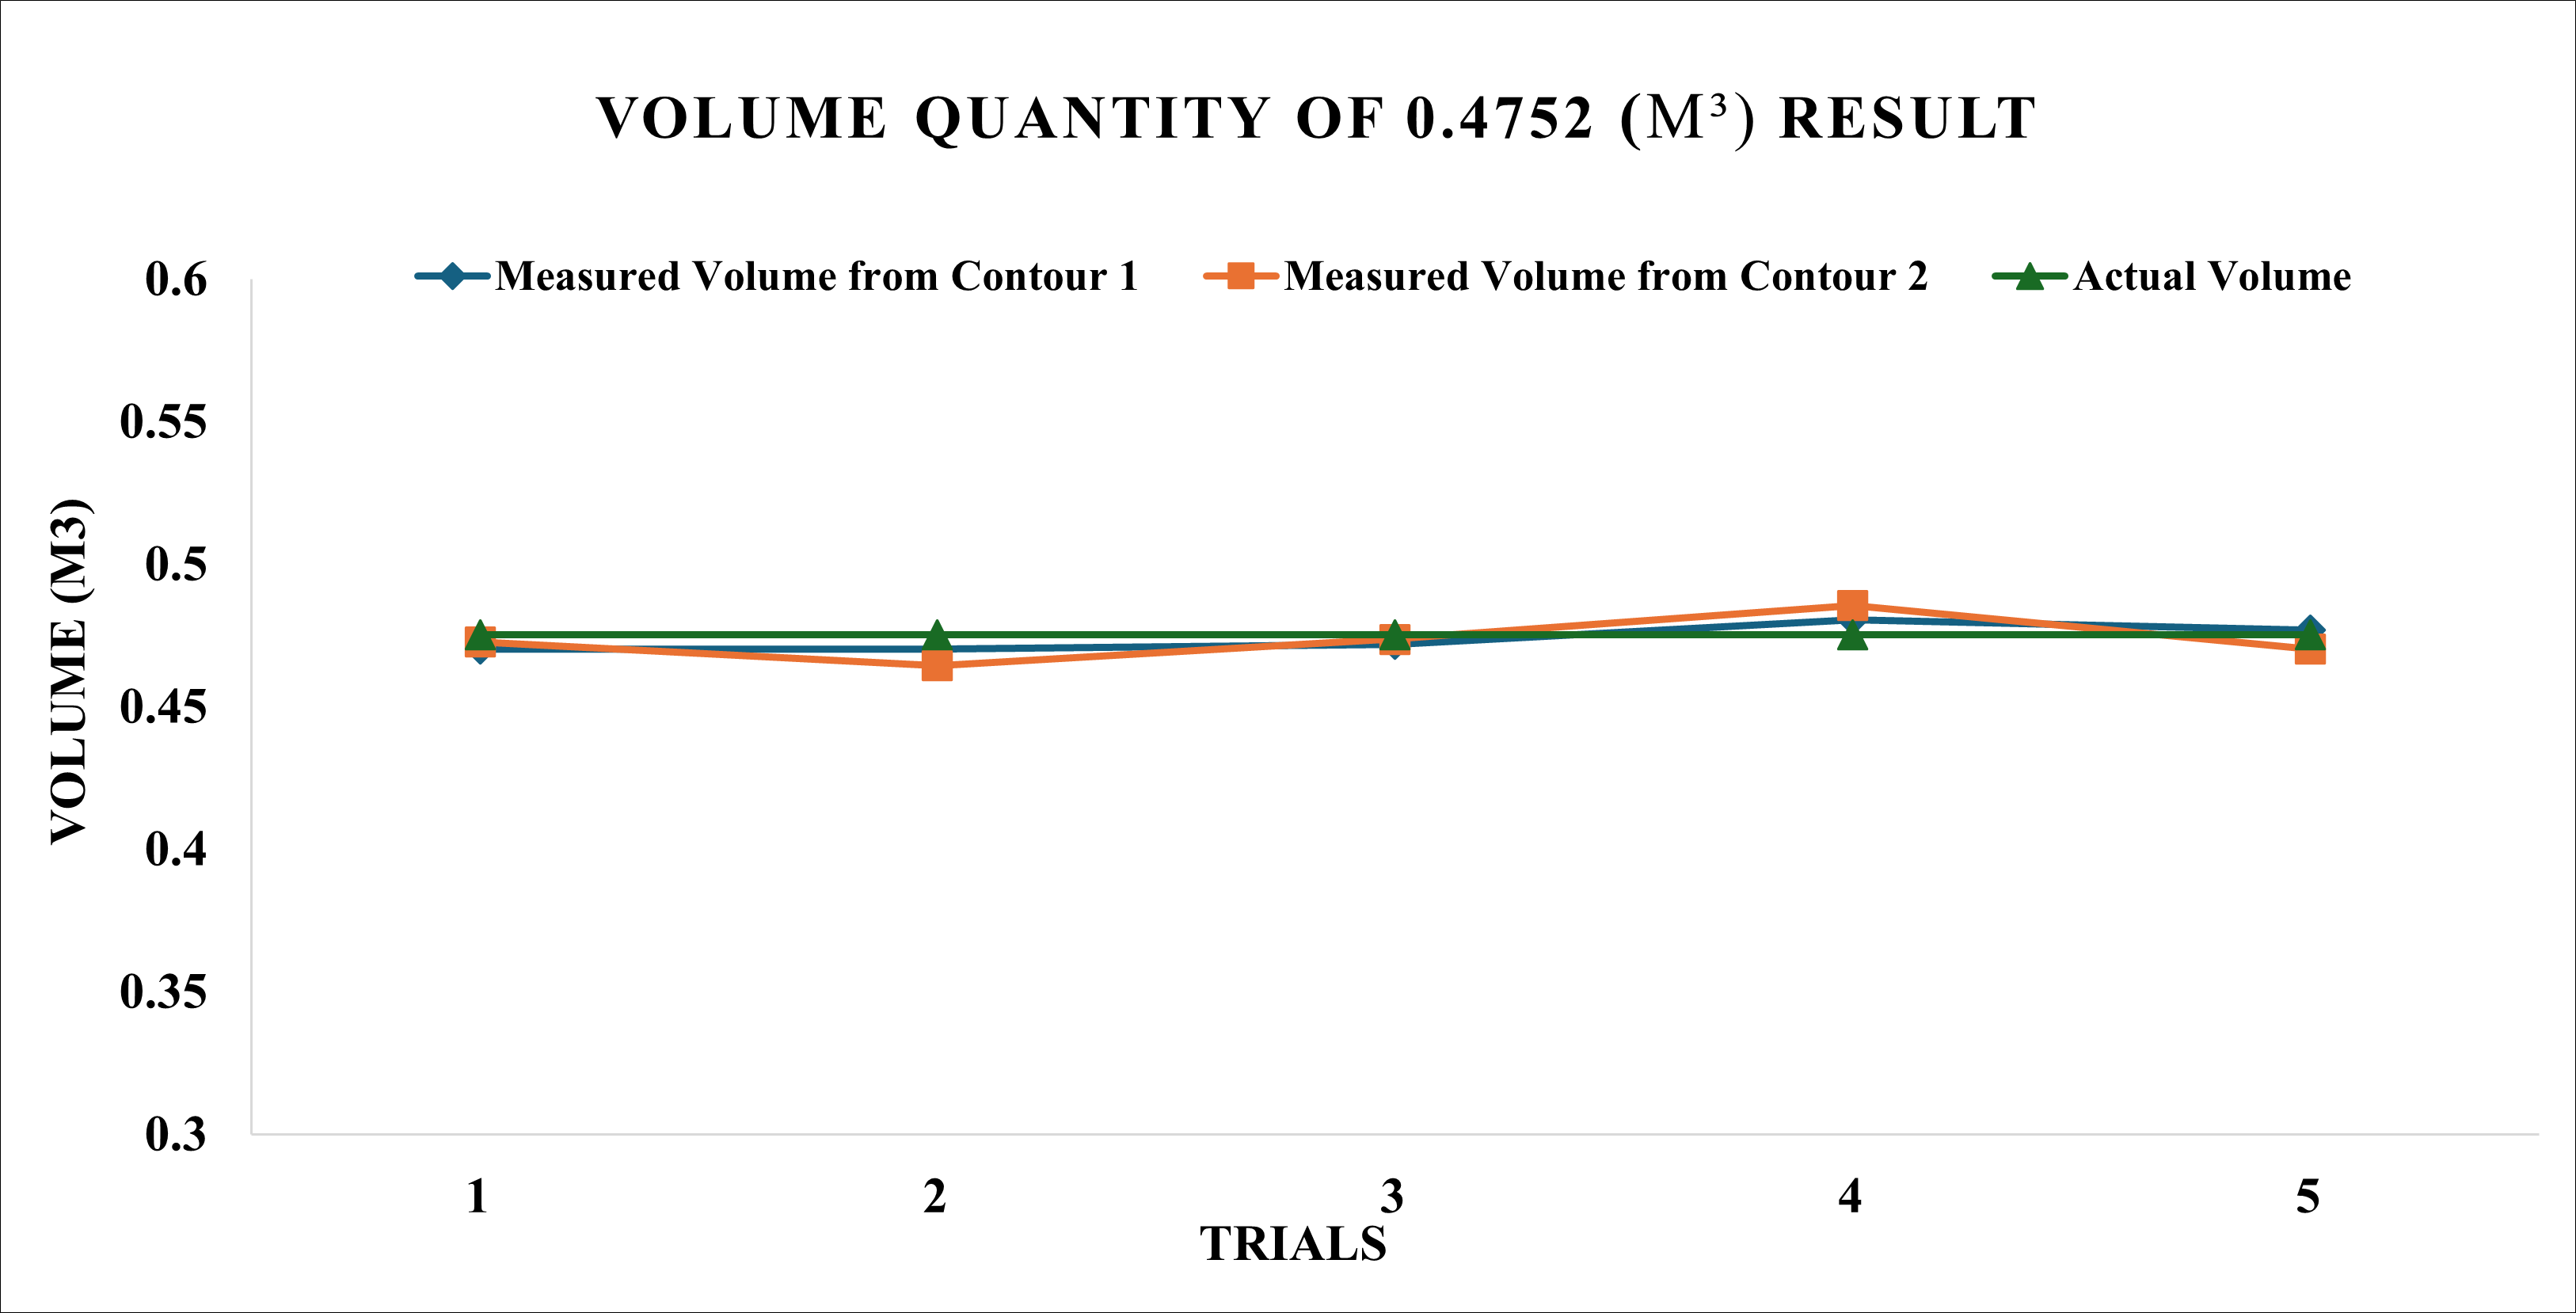
\includegraphics[width=0.8\textwidth]{Figures/test-case-2-2-graph}
	      %       \caption{Distribution of the Measured Volumes of two Contours}
	      %       \label{ch4:fig:test-case-2-2-graph}
	      %   \end{figure}

	      Based on the conducted ANOVA test and the statistic analysis table can be seen in Appendix \ref{appen:c} table \ref{table-anova-2}, there is no statistical difference for the 0.4752 $m^3$ level volume measurement according to the actual volume and those with different contours measured by the system with p value greater that 0.05.

	      %The results from test 2 gathered an average measured volume of 0.47407038 $m^{3}$ and 0.4733912158 $m^{3}$, a deviation of 0.00406 $m^{3}$ and 0.00691 $m^{3}$ from contour 1 and 2 respectively. Contour 1 achieved a MAPE of 0.8432\%, while the contour 2 have a MAPE of 1.2549\%. Overall, test 2 gathered an average measured volume with uncertainty of 0.47373 $\pm$ 0.0105 $m^{3}$ and an average MAPE of 1.04912\%. \\

	\item \textbf{Storage Bin Filled with 0.7128 $m^3$ of Flour}

	      A volume of 0.7128 $m^3$ was filled in the storage bin. Figure \ref{ch4:fig:test_2-3_contours} illustrates the actual flour surface contours along with the scanned point cloud contour by the system. The measured volumes across the two contours and the distribution of the data are presented in table \ref{table:test_case_2-2_results}.% and figure \ref{ch4:fig:test-case-2-3-graph}. \\
	      \\
	      \begin{figure}[H]
		      \centering
		      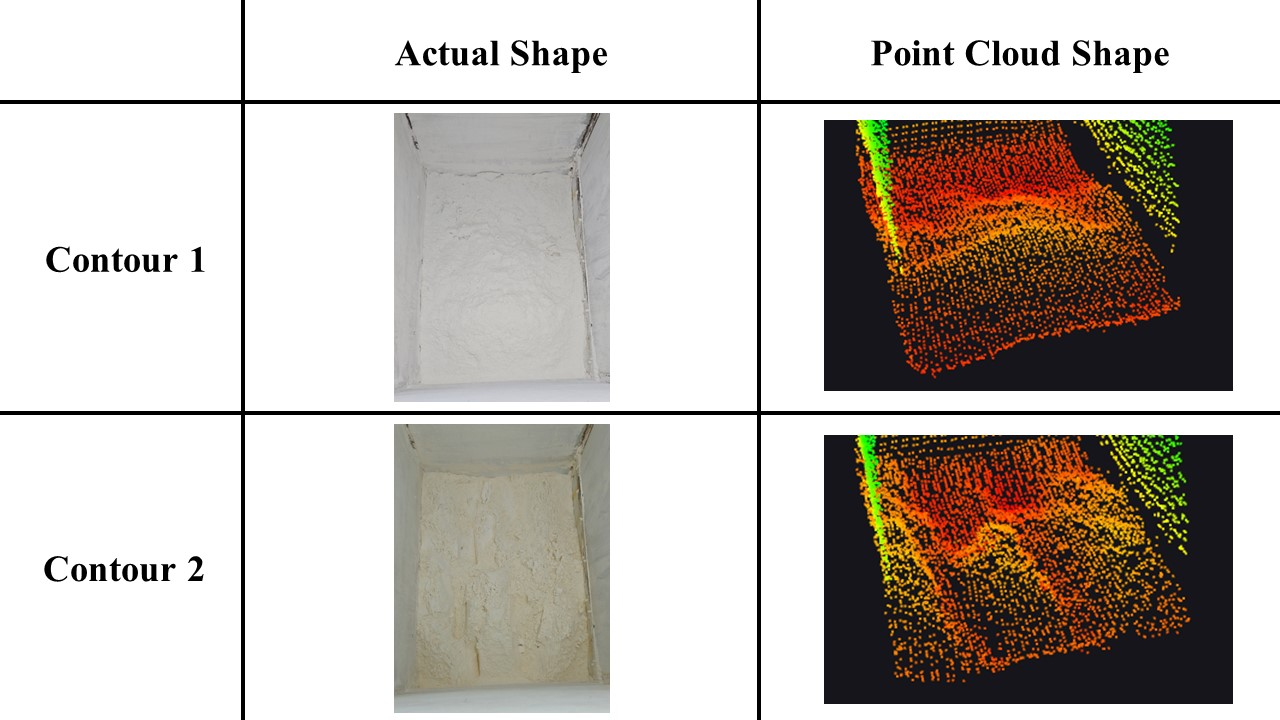
\includegraphics[width=0.8\textwidth]{Figures/test_2-3_contours}
		      \caption{Actual and Point Cloud Surface Contour of Test 3}
		      \label{ch4:fig:test_2-3_contours}
	      \end{figure}

	      The table \ref{table:test_case_2-3_results} presents the calibration results of volume measurements of the system across two contours, compared against a known volume of 0.7128 m³ filled in the flour bin. Over five trials, Contour 1 gathered an average measured volume of 0.7178206 m³, slightly higher estimation to the known volume. The Contour 2 gathered an average measured volume of 0.7202706 m³, also slightly higher estimation to the known volume. Both contours show minor variations, with Contour 1 being marginally closer to the known volume on average. \\

	      \begin{table}[H]
		      \centering
		      \begin{threeparttable}
			      \caption{Volume Measurements Calibration Result of the System Across Two Contours with A Known Volume of 0.7128 $m^3$}
			      \label{table:test_case_2-3_results}
			      \begin{tabular}{l c c r}
				      \toprule
				      \textbf{Trials} & \multicolumn{2}{c}{\textbf{Measured Volume ($m^{3}$)}} & \textbf{Known Volume} ($m^{3}$)          \\
				      {}              & Contour 1                                              & Contour 2                       & {}     \\ \midrule
				      1               & 0.716327                                               & 0.725803                        & 0.7128 \\
				      2               & 0.706001                                               & 0.724873                        & 0.7128 \\
				      3               & 0.720251                                               & 0.729404                        & 0.7128 \\
				      4               & 0.71687                                                & 0.715844                        & 0.7128 \\
				      5               & 0.729654                                               & 0.705429                        & 0.7128 \\ \midrule
				      Average         & 0.7178206                                              & 0.7202706                       & {}     \\ \bottomrule
			      \end{tabular}
		      \end{threeparttable}
	      \end{table}

	      %   \begin{figure}[H]
	      %       \centering
	      %       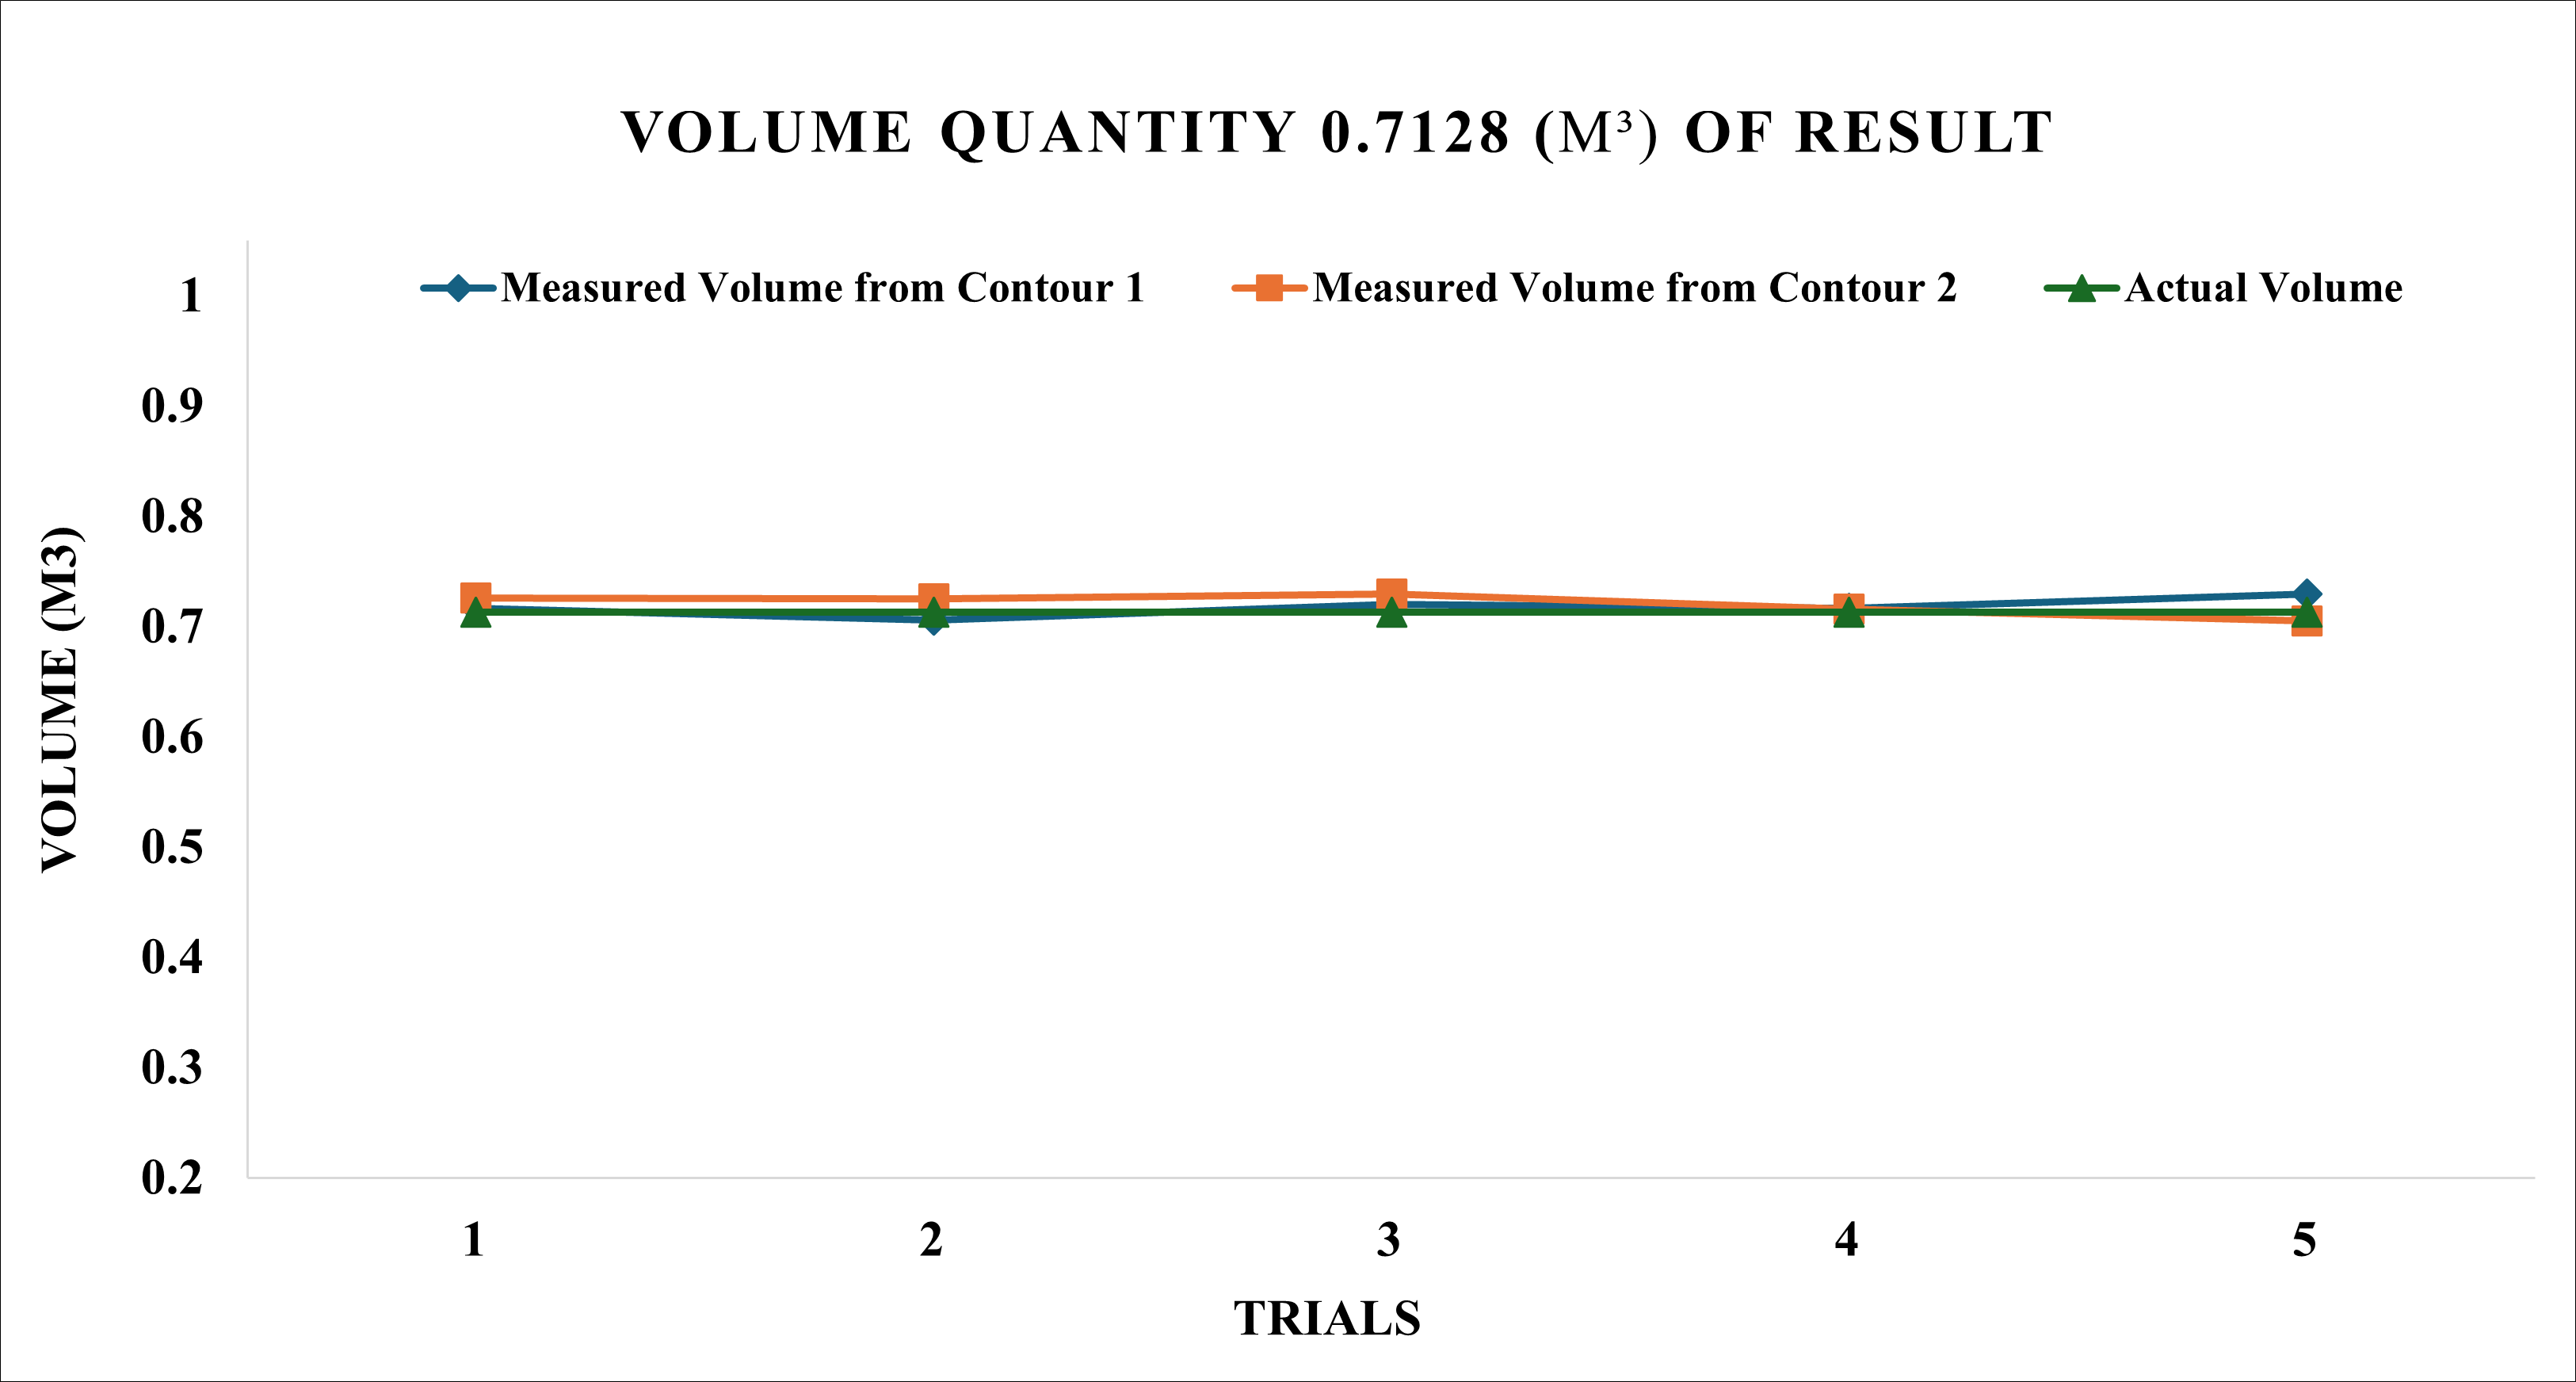
\includegraphics[width=0.8\textwidth]{Figures/test-case-2-3-graph}
	      %       \caption{Distribution of the Measured Volume of two Contours}
	      %       \label{ch4:fig:test-case-2-3-graph}
	      %   \end{figure}


	      %The results from test 3 gathered an average measured volume of 0.7178206 $m^{3}$ and 0.7202706 $m^{3}$, a deviation of 0.0076 $m^{3}$ and 0.0086 $m^{3}$ from contour 1 and 2 respectively. Contour 1 achieved a MAPE of 1.08588\%, while the contour 2 have a MAPE of 1.4617\%. Overall, Test 3 gathered an average measured volume with uncertainty of 0.719 $\pm$ 0.008239 $m^{3}$ and a MAPE of 1.27379\%. \\

	      Based on the conducted ANOVA test and the statistic analysis table can be seen in Appendix \ref{appen:c} table \ref{table-anova-2}, there is no statistical difference for the 0.7128 $m^3$ level volume measurement according to the actual volume and those with different contours measured by the system with p value greater that 0.05.
\end{enumerate}

\subsubsection{Volume Measurement Using the System and Sounding Method Result}
The results of the comparison are summarized in table \ref{ch4:tab:comparision-system-sounding}. The table presents the measured volumes using both methods for each contour shape and the percentage difference between them. The graph shown in \ref{ch4:fig:system-and-sounding-method} represents the distribution of volumes obtained from two different methods (system and sounding) for five contour trials. The actual testing images and scanned point cloud of the system can be seen in Appendix \ref{appen:b} under System and Sounding Method Actual Testing section. \\

\begin{figure}[H]
	\centering
	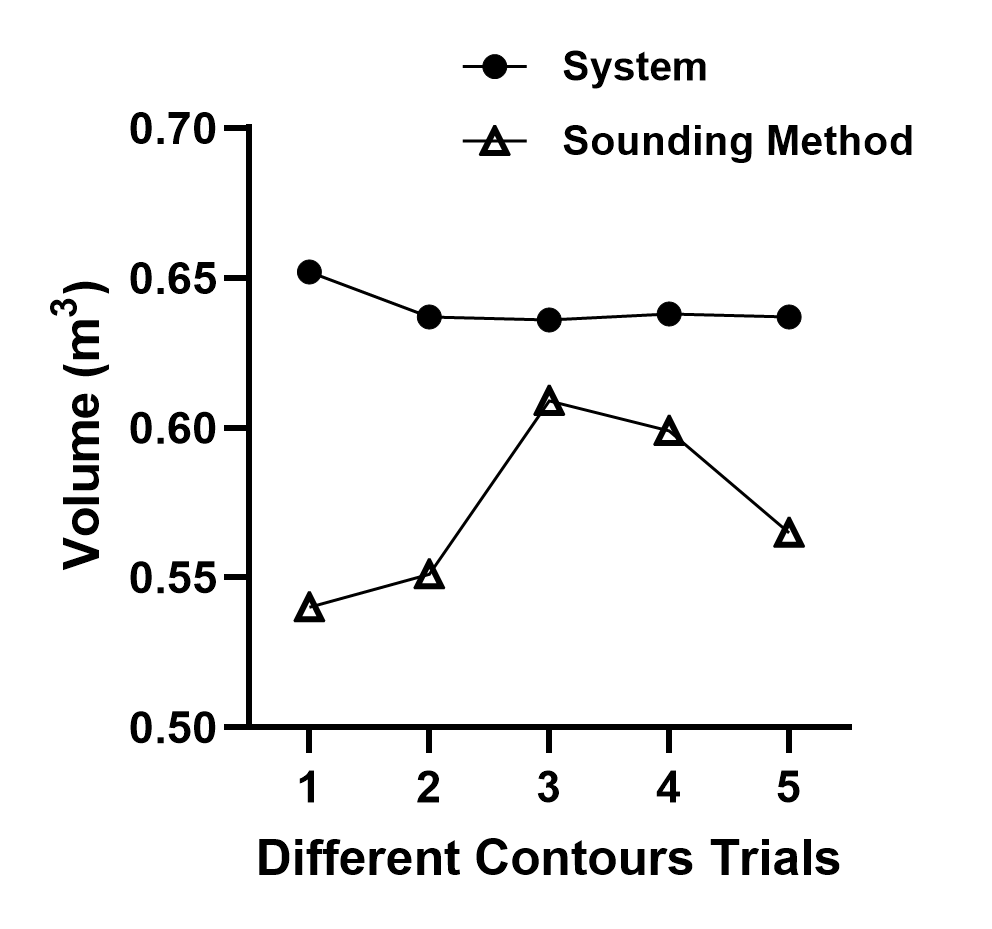
\includegraphics[width=0.7\textwidth]{Figures/system-and-sounding-method}
	\caption{Distribution of volume measurements obtained from the system and sounding}
	\label{ch4:fig:system-and-sounding-method}
\end{figure}

The table \ref{ch4:tab:comparision-system-sounding} compares volume measurements using the system and the traditional sounding method against an actual volume of 0.639 m³ across five trials each trials changed the contour surface of the flour. The measured volumes using the scanner system range from 0.636 m³ to 0.642 m³, with an average of 0.640 m³, closely matching the actual volume. The sounding method measurements range from 0.540 m³ to 0.609 m³, with an average of 0.573 m³, which is noticeably lower than the actual volume. This indicates that the 3D point cloud scanner system provides measurements that are much closer to the actual volume compared to the traditional sounding method. \\


\begin{table}[H]
	\centering
	\begin{threeparttable}
		\caption{Comparison of Volume Measurement Using the 3D Point Cloud Scanner System and Traditional Sounding Method for Different Surface Contours}
		\label{ch4:tab:comparision-system-sounding}
		\begin{tabular}{l c c r}
			\toprule
			\textbf{Trials} & \multicolumn{2}{c}{\textbf{Measured Volume ($m^{3}$)}} & \textbf{Actual Volume} ($m^{3}$)         \\
			{}              & System                                                 & Sounding Method                  & {}    \\ \midrule
			1               & 0.642                                                  & 0.540                            & 0.639 \\
			2               & 0.637                                                  & 0.551                            & 0.639 \\
			3               & 0.636                                                  & 0.609                            & 0.639 \\
			4               & 0.638                                                  & 0.599                            & 0.639 \\
			5               & 0.637                                                  & 0.565                            & 0.639 \\ \midrule
			Average         & 0.640                                                  & 0.573                            & {}    \\ \bottomrule
		\end{tabular}
	\end{threeparttable}
\end{table}

The comparison results demonstrate that the 3D Point Cloud Scanner System provides volume measurements that are consistent with those obtained using the traditional sounding method, regardless of the surface contour shape. The percentage differences between the two methods were minimal, indicating a high level of agreement.

The statistical analysis conducted for the comparison in table \ref{ch4:tab:comparision-system-sounding} is shown in appendix \ref{appen:c}, suggests since the p-value is less than 0.05, there is strong evidence to suggest that there is a significant difference between the sample mean of the sounding method data and the population mean of the system data. In other words, the sounding method measurements are significantly different from the system volume measurements.

%\subsection{Discussion}

%%%The test results demonstrate the effectiveness and accuracy of the developed 3D-PCSS in measuring the volume of both empty and filled storage bins. The system consistently provided reliable measurements across multiple trials and scenarios, validating its suitability for practical applications in various industries. Further analysis of the data collected revealed minor discrepancies between the measured and actual volumes, which can be attributed to factors such as sensor calibration and environmental conditions. Overall, the system performed satisfactorily and met the objectives set forth in this study. \\

%%%%%%%%%%%%%%%%%%%%%%%%%%%%%%%%%%%%%%%%%%%%%%

% \subsubsection*{Test Case 2.2: Storage Bin Filled to 47.2\% of Maximum Capacity}

% \begin{figure}[H]
% 	\centering
% 	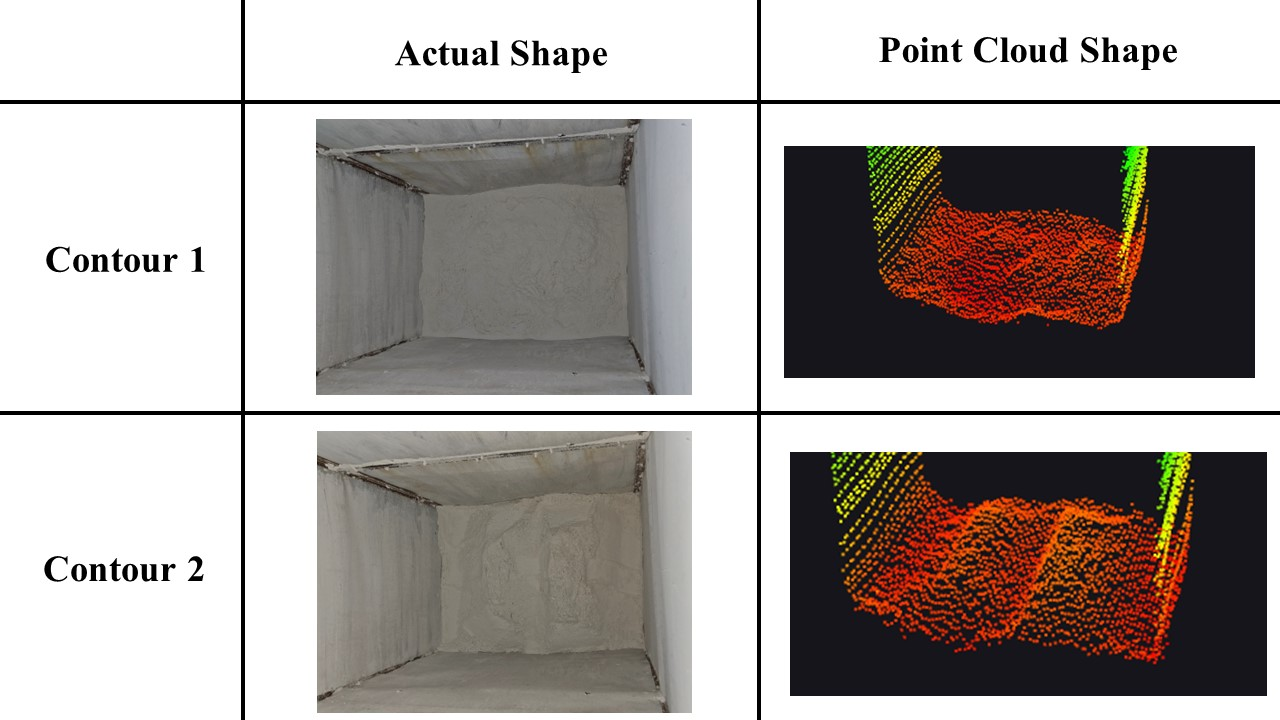
\includegraphics[width=0.8\textwidth]{Figures/test_2-2_contours}
% 	\caption{Different Flour Surface Contour of Test 2.2}
% 	\label{ch4:fig:test_2-2_contours}
% \end{figure}
% \begin{table}[H]
% 	\centering
% 	\caption{Test Case 2.2 Result}
% 	\label{table:test_case_2-2_results}
% 	\begin{tabular}{l c c r}
% 		\toprule
% 		\textbf{Trials} & \multicolumn{2}{c}{\textbf{Measured Volume ($m^{3}$)}} & \textbf{Actual Volume} ($m^{3}$)          \\
% 		{}              & Contour 1                                              & Contour 2                        & {}     \\ \midrule
% 		1               & 0.470418                                               & 0.472914                         & 0.4752 \\
% 		2               & 0.470279                                               & 0.464461                         & 0.4752 \\
% 		3               & 0.472061                                               & 0.473782                         & 0.4752 \\
% 		4               & 0.4805594                                              & 0.485587                         & 0.4752 \\
% 		5               & 0.4770345                                              & 0.470211                         & 0.4752 \\ \midrule
% 		Average         & 0.47407038                                             & 0.473391                         & {}     \\ \bottomrule
% 	\end{tabular}
% \end{table}

% \begin{figure}[H]
% 	\centering
% 	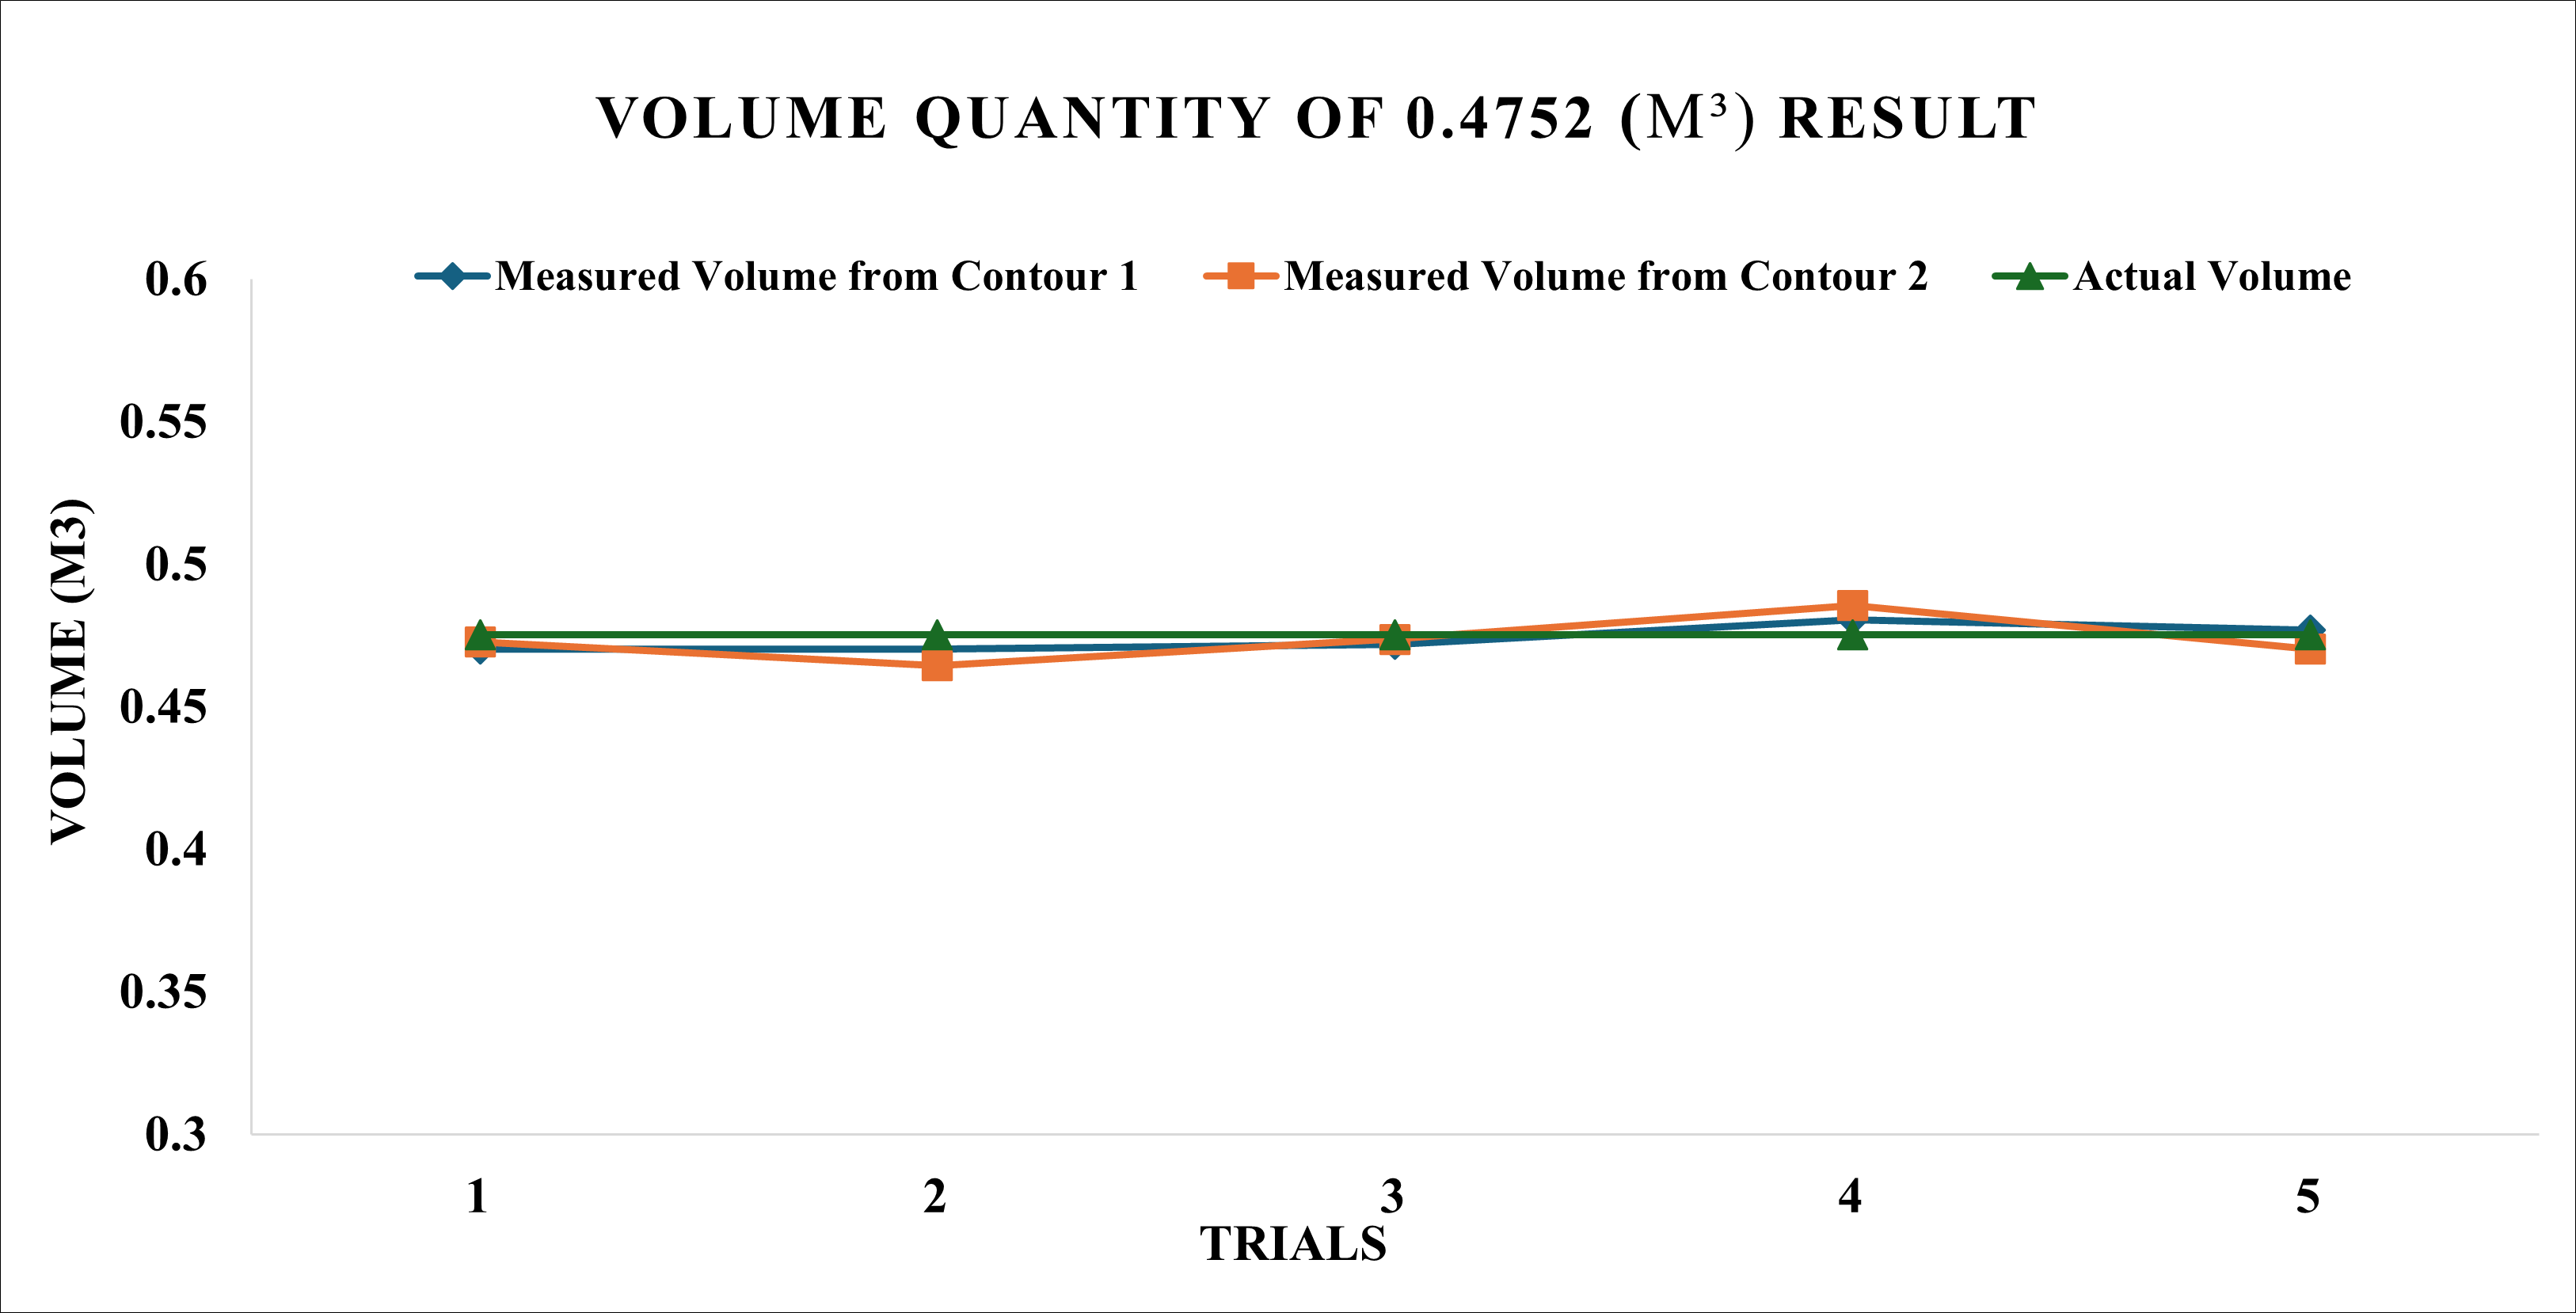
\includegraphics[width=0.8\textwidth]{Figures/test-case-2-2-graph}
% 	\caption{Distribution of the Measured Volume on Test Case 2.2}
% 	\label{ch4:fig:test-case-2-2-graph}
% \end{figure}

% The results from Test Case 2.2 gathered an average measured volume of 0.47407038 $m^{3}$ and 0.4733912158 $m^{3}$ and a deviation of 0.00406 $m^{3}$ and 0.00691 $m^{3}$ from contour 1 and 2 respectively. Contour 1 achieved a MAPE of 0.8432\%, while the contour 2 have a MAPE of 1.2549\%. Overall, Test Case 2.2 gathered an average measured volume with a standard deviation of 0.47373 $\pm$ 0.00568 $m^{3}$ and a MAPE of 1.04912\%.

% \subsubsection*{Test Case 2.3: Storage Bin Filled to 70.37\% of Maximum Capacity}
% \begin{figure}[H]
% 	\centering
% 	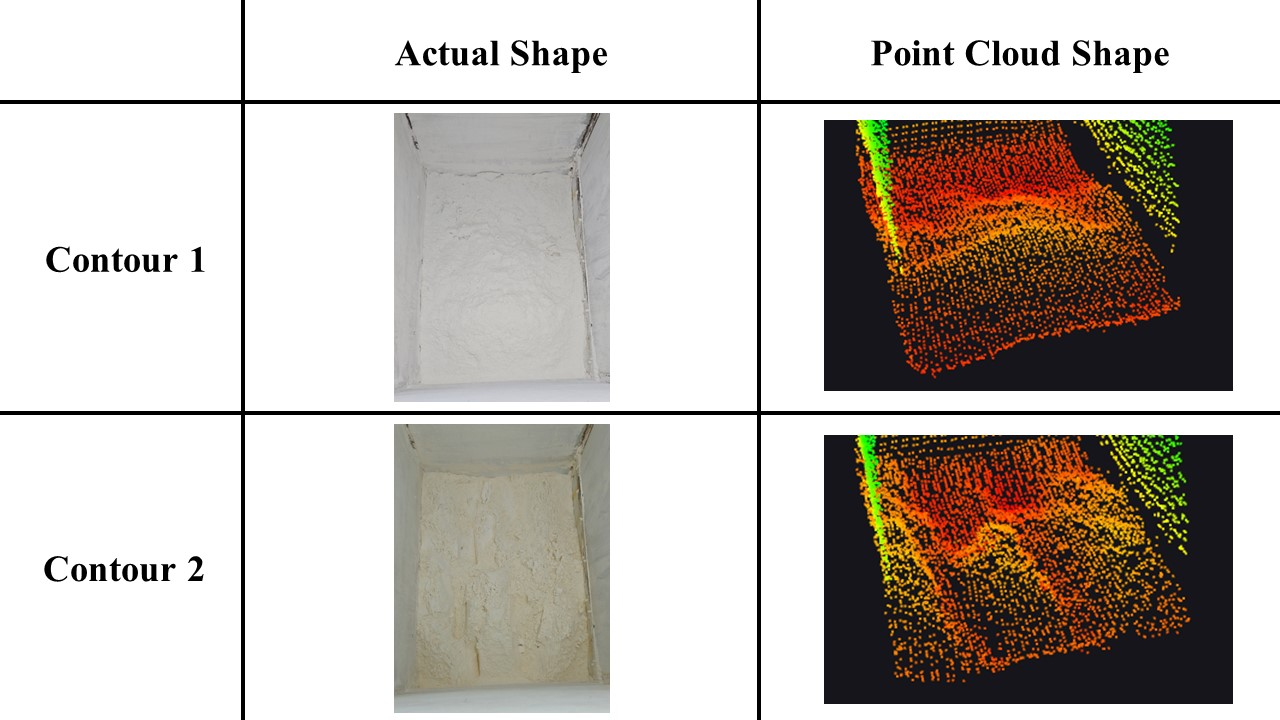
\includegraphics[width=0.8\textwidth]{Figures/test_2-3_contours}
% 	\caption{Different Flour Surface Contour of Test 2.3}
% 	\label{ch4:fig:test_2-3_contours}
% \end{figure}

% \begin{table}[H]
% 	\centering
% 	\caption{Test Case 2.3 Result}
% 	\label{table:test_case_2-3_results}
% 	\begin{tabular}{l c c r}
% 		\toprule
% 		\textbf{Trials} & \multicolumn{2}{c}{\textbf{Measured Volume ($m^{3}$)}} & \textbf{Actual Volume} ($m^{3}$)          \\
% 		{}              & Contour 1                                              & Contour 2                        & {}     \\ \midrule
% 		1               & 0.716327                                               & 0.725803                         & 0.7128 \\
% 		2               & 0.706001                                               & 0.724873                         & 0.7128 \\
% 		3               & 0.720251                                               & 0.729404                         & 0.7128 \\
% 		4               & 0.71687                                                & 0.715844                         & 0.7128 \\
% 		5               & 0.729654                                               & 0.705429                         & 0.7128 \\ \midrule
% 		Average         & 0.7178206                                              & 0.7202706                        & {}     \\ \bottomrule
% 	\end{tabular}
% \end{table}

% \begin{figure}[H]
% 	\centering
% 	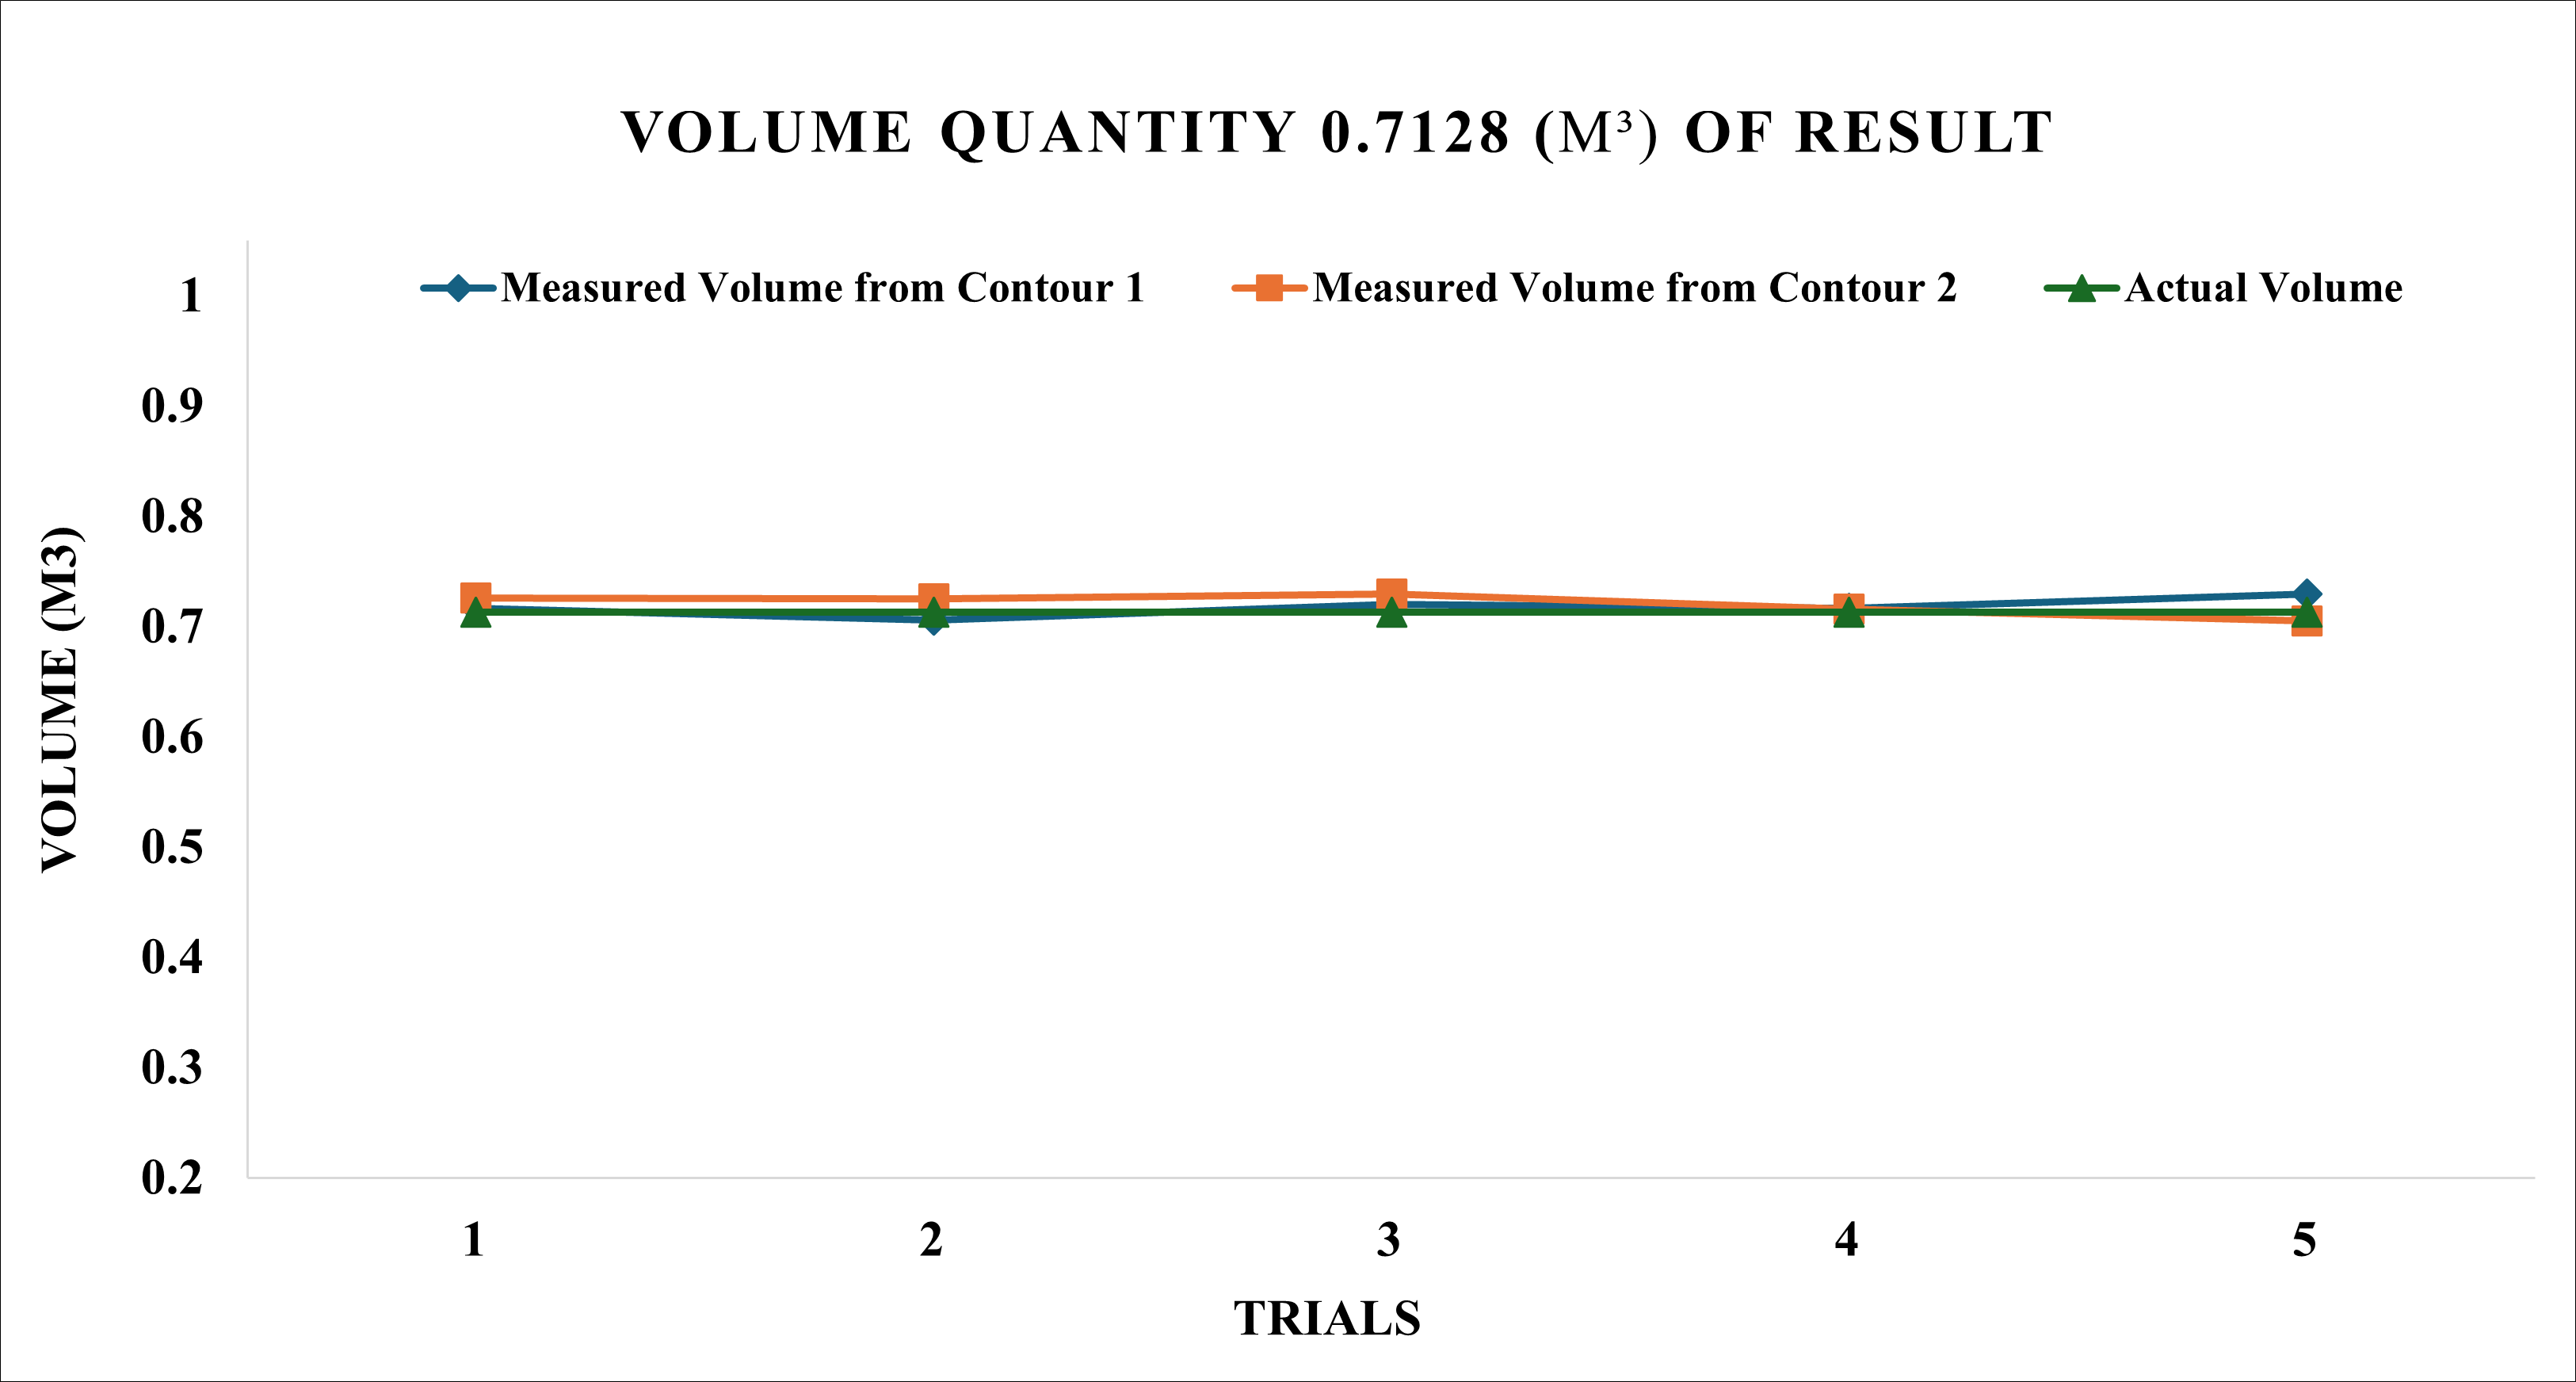
\includegraphics[width=0.8\textwidth]{Figures/test-case-2-3-graph}
% 	\caption{Distribution of the Measured Volume on Test Case 2.3}
% 	\label{ch4:fig:test-case-2-3-graph}
% \end{figure}


% The results from Test Case 2.3 gathered an average measured volume of 0.7178206 $m^{3}$ and 0.7202706 $m^{3}$ and a deviation of 0.0076 $m^{3}$ and 0.0086 $m^{3}$ from contour 1 and 2 respectively. Contour 1 achieved a MAPE of 1.08588\%, while the contour 2 have a MAPE of 1.4617\%. Overall, Test Case 2.3 gathered an average measured volume with a standard deviation of 0.719 $\pm$ 0.008239 $m^{3}$ and a MAPE of 1.27379\%.


%\subsection{Summary of the Conducted Test Cases}
% \begin{itemize}
% 	\item \textbf{Summary of the Conducted Test Cases:}
% \end{itemize}

% \begin{table}[H]
% 	\centering
% 	\caption{Summary of the of Test Case 2}
% 	\label{ch4:tab:test-cases-summary}
% 	\begin{tabular}{l l c c r}
% 		\toprule
% 		\multicolumn{2}{l}{\textbf{Test Cases}} & \textbf{\thead{Average Measured Volume                                                    \\ with Uncertainty ($m^{3}$)}} & \textbf{\thead{Average \\ MAPE (\%)}} & \textbf{\thead{Average \\ Standard Deviation ($m^{3}$)}}                \\ \midrule

% 		\multicolumn{2}{l}{1}                   & 1.009189 $\pm$ 0.0155                  & 0.5993776            & 0.007835601               \\

% 		{}                                      & 1                                      & 0.0595 $\pm$ 0.00065 & 0.71633     & 0.000453946 \\

% 		2                                       & 2                                      & 0.47373 $\pm$ 0.0105 & 1.04912     & 0.005489525 \\

% 		{}                                      & 3                                      & 0.719 $\pm$ 0.0121   & 1.27379     & 0.008130395 \\ \midrule

% 		Average                                 & {}                                     & {}                   & 0.909655    & 0.005477367 \\ \bottomrule
% 	\end{tabular}
% \end{table}

% The table \ref{ch4:tab:test-cases-summary} summarizes the two test cases conducted. The system achieved an average MAPE of 0.909655\% and average Standard Deviation of 0.005477367 $m^3$.

\subsection{System Evaluation}
The system evaluation section provides a comprehensive assessment of the 3D Point Cloud Scanner System's performance based on the data obtained from various testing procedures.

\subsubsection{LiDAR Calibration Evaluation}
The evaluation of the LiDAR device and servo calibration revealed consistent performance across different ranges. The highest Mean Absolute Error (MAE) of 0.0351 meters was observed at a distance of 3 meters, while the lowest MAE of 0.01616 meters was recorded at 1.5 meters. Additionally, the average Standard Deviation of 0.0103 meters across the five different distances signifies consistent precision in measurements. These results demonstrate the accurate and precise performance of the LiDAR device in capturing range data across varying distances.

\subsubsection{Servo Calibration Evaluation}
The evaluation of the servo calibration revealed consistent performance across different angles. The highest Mean Absolute Error (MAE) was 0.6 degrees, while the lowest MAE was 0.2 degrees. These results indicate reliable performance in accurately positioning the servo motor, ensuring precise control over the scanning mechanism of the system.

\subsubsection{Empty Storage Volume Measurement}
The average measured volume across all trials was determined to be 1.00919 $m^{3}$, with an uncertainty of $\pm$ 0.0155 $m^{3}$. The gathered Mean Absolute Percentage Error (MAPE) was calculated to be 0.599377608 \%, indicating the system's performance in accurately estimating the volume relative to the actual volume.

Additionally, the standard deviation of the measured volumes was determined to be 0.007835601 $m^{3}$, presenting consistency and precision of the system's volume measurements across multiple trials.

\subsubsection{Different Volume Quantity Measurement}

The system's performance achieved an average MAPE across the different volume quantity filled in the storage bin of 1.01308 \% and an average standard deviation 0.004691289 $m^3$, across the three conducted tests. This indicates that the system shows a consistent level of accuracy in measuring the volume of flour across different quantities. The average MAPE value of 1.01308\% suggests a minor deviation from the actual volume, which is within an acceptable range for the intended application. Additionally, the average standard deviation of 0.004691289 $m^3$ reflects the precision and consistency of the system's volume measurements. Overall, these results demonstrate the system's capability to accurately and reliably measure the volume of flour in varying storage capacities, providing valuable insights for its practical implementation and use.

% \subsubsection*{Summary of Test Case 2 Result}
% \begin{table}[H]
% 	\centering
% 	\caption{Summary of the 3 Different Volume Quantity Test}
% 	\label{ch4:tab:test-2-summary}
% 	\begin{tabular}{l c c r}
% 		\toprule
% 		\textbf{Test} & \textbf{\thead{Average Measured Volume                         \\ with Uncertainty ($m^{3}$)}} & \textbf{\thead{Average \\ MAPE (\%)}} & \textbf{\thead{Average \\ Standard Deviation ($m^{3}$)}} \\ \midrule

% 		1             & 0.0595 $\pm$ 0.00065                   & 0.71633 & 0.000453946 \\

% 		2             & 0.47373 $\pm$ 0.0105                   & 1.04912 & 0.005489525 \\

% 		3             & 0.719 $\pm$ 0.0121                     & 1.27379 & 0.008130395 \\ \midrule

% 		Average       & {}                                     & 1.01308 & 0.004691289 \\ \bottomrule
% 	\end{tabular}
% \end{table}

\subsubsection{Comparison Evaluation of the System and Sounding Method}

These results validate the accuracy of the overall performance of the system and suggest that it is a reliable alternative to the traditional sounding method for measuring the volume of flour in storage bins. The system's ability to provide consistent and accurate measurements across different surface contours, combined with its automation for estimation of the volume, offers significant advantages over manual methods, particularly in terms of efficiency and reduction of human error.

% \subsubsection{Overall System Evaluation}
% The table \ref{ch4:tab:test-cases-summary} summarizes the two volume measurement test conducted. The system achieved an average MAPE of 0.909655\% and average Standard Deviation of 0.005477367 $m^3$.

% \begin{table}[H]
% 	\centering
% 	\caption{Summary of the two Volume Measurement Test}
% 	\label{ch4:tab:test-cases-summary}
% 	\begin{tabular}{l l c c r}
% 		\toprule
% 		\multicolumn{2}{l}{\textbf{Test Cases}} & \textbf{\thead{Average Measured Volume                                                    \\ with Uncertainty ($m^{3}$)}} & \textbf{\thead{Average \\ MAPE (\%)}} & \textbf{\thead{Average \\ Standard Deviation ($m^{3}$)}}                \\ \midrule

% 		\multicolumn{2}{l}{1}                   & 1.009189 $\pm$ 0.0155                  & 0.5993776            & 0.007835601               \\

% 		{}                                      & 1                                      & 0.0595 $\pm$ 0.00065 & 0.71633     & 0.000453946 \\

% 		2                                       & 2                                      & 0.47373 $\pm$ 0.0105 & 1.04912     & 0.005489525 \\

% 		{}                                      & 3                                      & 0.719 $\pm$ 0.0121   & 1.27379     & 0.008130395 \\ \midrule

% 		Average                                 & {}                                     & {}                   & 0.909655    & 0.005477367 \\ \bottomrule
% 	\end{tabular}
% \end{table}

% Based on the summarized results, the system exhibited considerable performance in accurately measuring the volume of the flour storage bins. With an average Mean Absolute Percentage Error (MAPE) of 0.909655\%, the system demonstrated a relatively low level of error, remaining below the 1\% threshold. The observed errors ranged from 0.5993776\% to 1.27379\% from measured volume of 0.719 $\pm$ 0.0121 $m^3$ and 1.009189 $\pm$ 0.0155 $m^3$ respectively, indicating consistency across different volume quality.

% The average Standard Deviation achieved by the system with a value of 0.005477367 $m^3$. This indicates that the measurements of the system throughout the test are clustered closely, thus the precision of the system measurement is considerably high.